\documentclass[letter]{article}
\usepackage[letterpaper]{geometry}
\usepackage{amsmath}
\usepackage{amsfonts}
\usepackage{amssymb}
\usepackage{graphicx}
\usepackage[inline]{enumitem}
\usepackage{amsfonts}
\usepackage{amssymb}
\usepackage{xparse}
\usepackage{ifthen}
\usepackage{graphicx}
\usepackage{caption}
\usepackage{subcaption}
\usepackage{color}
\usepackage{tikz}
\usepackage{fancyhdr}
\usepackage{calc}

\usepackage{pgfplots}
\pgfplotsset{compat=newest}
%\usepackage[hidelinks]{hyperref}
%\usepackage{wrapfig}


%%%
% Set up the margins to use a fairly large area of the page
%%%
\oddsidemargin=.2in
\evensidemargin=.2in
\textwidth=6in
\topmargin=-1.2in
\textheight=9.8in
\parskip=.07in
\parindent=0in

%%%
% Make the copyright notice appear in the footer
%%%
\pagestyle{fancy}
\rfoot{\footnotesize\it \copyright\,Jason Siefken, 2015 \ \makebox(30,5){\includegraphics[height=1.2em]{by-sa.pdf}}}
\renewcommand{\headrulewidth}{0pt}

%%%
% Custom enumerate environment Enum
% that incriments the problem number every time it is used.
%%%
\newcounter{EnumPrefix}
\newcounter{EnumSuffix}
\DeclareDocumentEnvironment{Enum}{o}{
	\ifthenelse{ \equal{#1}{resume} }{
		\begin{enumerate}[label={\footnotesize\arabic{EnumPrefix}}.\arabic*]
		\setcounter{enumi}{\value{EnumSuffix}}
	}{
		\stepcounter{EnumPrefix}\begin{enumerate}[label={\footnotesize\arabic{EnumPrefix}}.\arabic*]
	}
}{
	\setcounter{EnumSuffix}{\value{enumi}}
	\end{enumerate}
}

%%%
% Useful Linear Algebra macros
%%%
\newcommand{\ul}{$\underline{\phantom{xxx}}$}
\newcommand{\ull}{\underline{\phantom{xxx}}}
\newcommand{\xh}{{\hat {\mathbf x}}}
\newcommand{\yh}{{\hat {\mathbf y}}}
\newcommand{\zh}{{\hat {\mathbf z}}}
\newcommand{\R}{\mathbb{R}}
\newcommand{\Z}{\mathbb{Z}}
\newcommand{\N}{\mathbb{N}}
\newcommand{\proj}{\mathrm{proj}}
\newcommand{\Proj}{\mathrm{proj}}
\newcommand{\Perp}{\mathrm{perp}}
\renewcommand{\span}{\mathrm{span}\,}
\newcommand{\Span}{\mathrm{span}\,}
\newcommand{\Img}{\mathrm{img}\,}
\newcommand{\Null}{\mathrm{null}\,}
\newcommand{\Range}{\mathrm{range}\,}
\newcommand{\rref}{\mathrm{rref}}
\newcommand{\rank}{\mathrm{rank}}
\newcommand{\Rank}{\mathrm{rank}}
\newcommand{\nnul}{\mathrm{nullity}}
\newcommand{\mat}[1]{\begin{bmatrix}#1\end{bmatrix}}
\newcommand{\chr}{\mathrm{char}}
\newcommand{\url}[1]{#1}
\renewcommand{\d}{\mathrm{d}}

%%%
% Create a command that draws a horizontal line extending into the margin.
% If no argument is given, it prints the current problem number.
% Otherwise the argument is displayed (including a blank argument)
%%%

%\definecolor{barcolor}{rgb}{.2,.6,1.0}  % medium blue
\definecolor{barcolor}{rgb}{.1,.4,.5} % dark blue
\NewDocumentCommand{\sep}{o}{%
	\makebox(0,0){%
		\vspace{.1in}
		\hspace{-1.0in}
		\color{barcolor}{
			\makebox(0,10)[l]{\rule{1.4in}{.25pt}}
			\IfNoValueTF{#1}{
				\stepcounter{EnumPrefix}
				\makebox(0,0)[lt]{\arabic{EnumPrefix}}
				\addtocounter{EnumPrefix}{-1}
			}{
				\makebox(0,0)[lt]{\emph{#1}}
			}
		}
}\\*[0pt]}
% a \sep command to be used before a list.  Remove the extra spacing...
\newcommand{\sepl}{\sep \vspace{-.35in}}

\definecolor{defcolor}{rgb}{.05,.4,.15}
\newsavebox{\fminipagebox}
\newlength{\currentparskip}
\NewDocumentEnvironment{Def}{O{\fboxsep}}
 {
	 \renewcommand{\emph}[1]{{\color{defcolor} \textbf{\textit{##1}}}}
 	\setlength{\currentparskip}{\parskip}
	\makebox(0,0){%
			\vspace{.0in}
			\hspace{-.9in}
			\color{defcolor}{
				\makebox(0,-12)[lt]{\bf{Def}}
			}
	}
 \par\kern#1\noindent\begin{lrbox}{\fminipagebox}
  \begin{minipage}{\textwidth}\ignorespaces%
  \setlength{\parskip}{.4em}
}
 {\end{minipage}\end{lrbox}%
  \makebox[\textwidth]{%
    \kern\dimexpr-\fboxsep-\fboxrule\relax
    \fbox{\usebox{\fminipagebox}}%
    \kern\dimexpr-\fboxsep-\fboxrule\relax
  }\par\kern#1
  \setlength{\parskip}{\currentparskip}
 }
%\DeclareDocumentEnvironment{Def}{O{\textwidth} O{\fboxsep}}{
%	\makebox(0,0){%
%			\vspace{.0in}
%			\hspace{-.7in}
%			\color{defcolor}{
%				\makebox(0,10)[l]{\rule{1.0in}{.25pt}}
%				\makebox(0,0)[lt]{\emph{Def}}
%			}
%	}\\*
%	{\par\kern#2\noindent\begin{lrbox}{\fminipagebox}\begin{minipage}{#1}\ignorespaces}
%}{%
%	%\makebox(0,0){}	\newline
%	\hspace*{\fill}\\*
%	\makebox(0,0){%
%			\vspace{.2in}
%			\hspace{-.7in}
%			\color{defcolor}{
%				\makebox(0,10)[l]{\rule{1.0in}{.25pt}}
%			}
%	}
% \end{minipage}\end{lrbox}%
%  \makebox[#1]{%
%    \kern\dimexpr-\fboxsep-\fboxrule\relax
%    \fbox{\usebox{\fminipagebox}}%
%    \kern\dimexpr-\fboxsep-\fboxrule\relax
%  }\par\kern#2
%	\vspace{-.2in}
%}



%%%
% Start the document!
%%%
\begin{document}
\pagestyle{empty}

\begin{center}
{\huge\bf Inquiry Based Linear Algebra}\\

\vspace{.7in}
{
\it \copyright\,Jason Siefken, 2015 \\
Creative Commons By-Attribution Share-Alike\, \makebox(30,5){\includegraphics[height=1.2em]{by-sa.pdf}}
}
\end{center}

\section*{About the Document}
This document was originally designed in the spring of 2015 to guide students
through an eleven week Linear Algebra course (Math 211, Linear Algebra for Scientists) at
the University of Victoria.  The order of topics closely follows that in {\it Linear
Algebra for Science and Engineering} second edition by Daniel Norman and Dan Wolczuk.

A typical class day using the problem-sets:
\begin{enumerate}
	\item {\bf Introduction by instructor.} This may involve giving a definition,
		a broader context for the day's topics, or answering questions.
	\item {\bf Students work on problems.} Students work individually or in pairs
		on the prescribed problem.  During this time the instructor moves around
		the room addressing questions that students may have and giving one-on-one
		coaching.
	\item {\bf Instructor intervention.} If most students have successfully solved the 
		problem, the instructor regroups the class by providing a concise 
		explanation so that everyone is ready to move to the next concept.  This
		is also time for the instructor to ensure that everyone has understood the
		main point of the exercise (since it is sometimes easy to do some computation
		while being oblivious to the larger context).

		If students are having trouble, the instructor can give hints to the group,
		and additional guidance to ensure the students don't get frustrated
		to the point of giving up.
	\item {\bf Repeat step 2.}
\end{enumerate}

Using this format, students are working (and happily so) most of the class.
Further, they are especially primed to hear the insights of the instructor, 
having already invested substantially into each problem.


These problem-sets strike a balance between concepts and computation, leaning towards
the conceptual side.  Two algorithms, \emph{row reduction} and \emph{determinant of
a matrix by cofactors}, are not introduced in these problem-sets.  Instead, students are
expected to learn them on their own and be prepared to apply them on problems in the
problem-set (these topics were left up to the students because of time constraints).
Further, not ever Linear Algebra definition is given in these problem-sets, since these
notes are not intended to replace a Linear Algebra textbook, but most definitions
are given to expedite the transition to new topics in the middle of class time.

{\bf License}  This document is licensed under the Creative Commons
By-Attribution Share-Alike License.  That means, you are free to use,
copy, and modify this document provided that you provide attribution
to the previous copyright holders and you release your derivative work 
under the same license.  Full text of the license is at \url{http://creativecommons.org/licenses/by-sa/4.0/}

If you modify this document, you may add your name to the copyright list.  Also,
if you think your contributions would be helpful to others, consider making a pull
requestion, or opening an \emph{issue} at 
\url{https://github.com/siefkenj/IBLLinearAlgebra}


%%%
% Start the Math!
%%%
\newpage
\setcounter{page}{1}
\pagestyle{fancy}

\section*{Vectors}

	\sep
	\begin{tikzpicture}[>=latex,scale=4]
		\draw[style=help lines] (0,0) (2,2);

		\draw[->,thick,black] (0,0) -- (135:1) node [left] {$\mathbf a$};
		\draw[->,thick,black] (0,0) -- (0,1) node [left] {$\mathbf b$};
		\draw[->,thick,black] (0,0) -- (45:1) node [above] {$\mathbf c$};
		\draw[->,thick,black] (0,0) -- (1,0) node [above] {$\mathbf d$};
		\draw (0,0) node [below] {$\mathbf o$};
		
		\draw[thick,blue,fill] (1,2) circle [radius=.02] node [below right,black] {$p$};
		\draw[thick,blue] (2,1) circle [radius=.02] node [below right,black] {$q$};

	\end{tikzpicture}

	Notice that all arrows in this diagram are the same length.
	We will call this length a \emph{unit}.
	\begin{Enum}
		\item Give directions from $\bf o$ to $p$ of
		the form ``Walk \ul units in the direction of arrow \ul, then 
		walk \ul units in the direction of arrow \ul.''

		\item Can you give directions with the two arrows you haven't
		used?  Give such directions, or explain why it cannot be done.

		\item Give directions from $\bf o$ to $q$.

		\item Can you give directions from $\bf o$ to $q$ using $\bf c$ and $\bf a$?
		Give such directions, or explain why it cannot be done.

	\end{Enum}
	

	\sep
	\begin{minipage}{.35\textwidth}
	\begin{tikzpicture}[>=latex,scale=4]
		\draw[style=help lines] (0,0) (1,2);

		\draw[->,thick,black] (0,0) -- (0,1) node [left] {$\yh$};
		\draw[->,thick,black] (0,0) -- (63.4:1) node [left] {$\mathbf c$};
		\draw[->,thick,black] (0,0) -- (1,0) node [above] {$\xh$};
		\draw (0,0) node [below] {$\mathbf o$};
		
		\draw[thick,blue,fill] (1,2) circle [radius=.02] node [below right,black] {$p$};

	\end{tikzpicture}
	\end{minipage}
	\begin{minipage}{.65\textwidth}
	We are going to start using a more mathematical notation
	for giving directions.  Our directions will now look like
	\[
		p = \ull\, \xh + \ull\, \yh
	\]
	which is read as ``To get to $p$ (=) go \ul units in the direction $\xh$ then (+) go \ul units in 
	the direction $\yh$.''

	\begin{Enum}
		\item What is the difference between $p = \ull\, \xh + \ull\, \yh$ and $p = \ull\, \yh + \ull\, \xh$?
		Can they both give valid directions?
		\item
		\begin{enumerate}
			\item Give directions to $p$ using the new notation. 
			\item Give directions to $p$ using $\bf c$.
			\item What is the distance from $\bf o$ to $p$ in units?
		\end{enumerate}
		\item
		\begin{enumerate}
			\item $r=1\bf c$.  Give directions from $\bf o$ to $r$ using $\xh$ and $\yh$.
			\item What is the distance from $\bf o$ to $r$?
		\end{enumerate}
		\item
		\begin{enumerate}
			\item $q=-2\xh+3\yh$; find the exact distance from $\bf o$ to $q$.
			\item $s=2\xh+\bf c$; find the exact distance from $\bf o$ to $s$.
		\end{enumerate}
	\end{Enum}
	\end{minipage}


	The vectors $\xh$ and $\yh$ are called the \emph{standard
	basis vectors} for $\R^2$ (the plane).  

\section*{Column Vector Notation}
	We previously wrote $q=-2\xh+3\yh$.  In column vector notation we write
	\[
		q=\begin{bmatrix}-2\\3\end{bmatrix}
	\]
	We may call $q$ either a \emph{vector} or a \emph{point}.  If we call $q$ a vector,
	we are emphasizing that $q$ gives direction of some sort.  If we call $q$ a point,
	we emphasize that $q$ is some absolute location in space. (What's the philosophical
	difference between a location in space and directions from the origin to said location?)

	\sep 
	$r=1\bf c$ and $s=2\xh+\bf c$ where $\bf c$ is the vector from before.
	\begin{Enum}
		\item Write $r$ and $s$ in column vector form.
	\end{Enum}

\section*{Sets and Set Notation}

	\begin{Def}
		A \emph{set} is a (possibly infinite) collection of items
		and is notated with curly braces (for example, $\{1,2,3\}$ is
		the set containing the numbers 1, 2, and 3).  We call the items in
		a set \emph{elements}.

		If $X$ is a set and $a$ is an element $X$, we may write $a\in X$,
		which is read ``$a$ is an element of $X$.''

		If $X$ is a set, a \emph{subset} $Y$ of $X$ (written $Y\subseteq X$)
		is a set such that every element of $Y$ is an element of $X$.

		We can define a subset using \emph{set-builder notation}.
		That is, if $X$ is a set, we can define the subset 
		\[
			Y= \{a\in X:\text{some rule involving }a\},
		\]
		which is read ``$Y$ is the set of $a$ in $X$ {\bf such that} some rule
		involving $a$ is true.''  If $X$ is intuitive, we may omit it and
		simply write $Y=\{a:\text{some rule involving }a\}$.  You may equivalently
		use ``$|$'' instead of ``$:$'', writing $Y=\{a\,|\,\text{some rule involving }a\}$.
	\end{Def}

	\begin{Def}
		Some common sets are
		\vspace{-1em}
		\begin{itemize}
			\item[] $\N=\{\text{natural numbers}\} = \{\text{non-negative whole numbers}\}$.
			\item[] $\Z=\{\text{integers}\} = \{\text{whole numbers, including negatives}\}$.
			\item[] $\R=\{\text{real numbers}\}$.
			\item[] $\R^n=\{\text{vectors in $n$-dimensional Euclidean space}\}$.
		\end{itemize}
	\end{Def}

	\sep
	\vspace{-2em}
	\begin{Enum}
		\item Which of the following are true?
		\begin{enumerate}
			\item $3\in\{1,2,3\}$.
			\item $4\in\{1,2,3\}$.
			\item ``b''$\in\{x:x\text{ is an English letter}\}$.
			\item ``\`o''$\in\{x:x\text{ is an English letter}\}$.
			\item $\{1,2\}\subseteq \{1,2,3\}$.
			\item For some $a\in\{1,2,3\}$, $a \geq 3$.
			\item For any $a\in\{1,2,3\}$, $a\geq 3$.
			\item $1\subseteq\{1,2,3\}$.
			\item $\{1,2,3\}=\{x\in\R:1\leq x\leq 3\}$.
			\item $\{1,2,3\}=\{x\in\Z:1\leq x\leq 3\}$.
		\end{enumerate}
	\end{Enum}

	\sep
		Write the following in set-builder notation
	\begin{Enum}
			\item The subset $A\subseteq \R$ of real numbers larger than $\sqrt{2}$.
			\item The subset $B\subseteq \R^2$ of vectors whose first coordinate
			is twice the second.
	\end{Enum}

	\begin{Def}
		Two common set operations are \emph{unions} and \emph{intersections}.  
		Let $X$ and $Y$ be sets.

		\hfill\begin{minipage}{\dimexpr\textwidth-3cm}
		\begin{itemize}
			\item[(union)] $X\cup Y = \{a:a\in X\text{ or }a\in Y\}$.
			\item[(intersection)] $X\cap Y = \{a: a\in X\text{ and }a\in Y\}$.
		\end{itemize}
		\end{minipage}
	\end{Def}

	\sep
	Let $X=\{1,2,3\}$ and $Y=\{2,3,4,5\}$ and $Z=\{4,5,6\}$.  Compute
	\begin{Enum}
		\item $X\cup Y$
		\item $X\cap Y$
		\item $X\cup Y\cup Z$
		\item $X\cap Y\cap Z$
	\end{Enum}

	\sep
	Draw the following subsets of $\R^2$.
	\begin{Enum}
		\item $V=\left\{\vec x\in\R^2:\vec x=\begin{bmatrix}0\\t\end{bmatrix}\text{ for some }t\in\R\right\}$.
		\item $H=\left\{\vec x\in\R^2:\vec x=\begin{bmatrix}t\\0\end{bmatrix}\text{ for some }t\in\R\right\}$.
		\item $J=\left\{\vec x\in\R^2:\vec x=t\begin{bmatrix}1\\1\end{bmatrix}\text{ for some }t\in\R\right\}$.
		\item $V\cup H$.
		\item $V\cap H$.
		\item Does $V\cup H=\R^2$?
	\end{Enum}



\section*{Dot Product}
	\vspace{-1cm}

	\begin{Def}
	If $\vec a=\begin{bmatrix}a_1\\ a_2\\ \vdots \\ a_n\end{bmatrix}$ and 
	$\vec b=\begin{bmatrix}b_1\\ b_2\\ \vdots \\ b_n\end{bmatrix}$ are two vectors in $n$-dimensional
		space, then the \emph{dot product} of $\vec a$ an $\vec b$ is
	\[
		\vec a\cdot\vec b = a_1b_1+a_2b_2+\cdots+a_nb_n.
	\]
	Equivalently, the dot product is defined by the geometric formula
	\[
		\vec a\cdot \vec b = \|\vec a\|\|\vec b\|\cos \theta
	\]
	where $\theta$ is the angle between $\vec a$ and $\vec b$.
	\end{Def}
	
	\pagebreak
	\sep
		Let $\vec a=\begin{bmatrix}1\\1\end{bmatrix}$, $\vec b=\begin{bmatrix}3\\2\end{bmatrix}$, and $\vec u=\begin{bmatrix}1\\2\\1\end{bmatrix}$.
	\vspace{-.5cm}
	\begin{Enum}
		\item 
		\begin{enumerate}	
			\item Draw a picture of $\vec a $ and $\vec b$.
			\item Compute $\vec a\cdot \vec b$.
			\item Find $\|\vec a\|$ and $\|\vec b\|$ and use your knowledge of
			the multiple ways to compute the dot product to find $\theta$,
			the angle between $\vec a$ and $\vec b$. Label $\theta$ on your picture.
		\end{enumerate}
		\item Draw the graph of $\cos$ and identify which angles make $\cos$ negative, zero,
		or positive.

		\item Draw a new picture of $\vec a$ and $\vec b$ and on that picture draw
		\begin{enumerate}	
			\item a vector $\vec c$ where $\vec c\cdot \vec a$ is negative.
			\item a vector $\vec d$ where $\vec d\cdot \vec a=0$ and $\vec d\cdot \vec b < 0$.
			\item a vector $\vec e$ where $\vec e\cdot \vec a=0$ and $\vec e\cdot \vec b>0$.
			\item Could you find a vector $\vec f$ where $\vec f\cdot \vec a=0$ and $\vec f\cdot \vec b=0$?
			Explain why or why not.
		\end{enumerate}

		\item Recall the vector $\vec u$ whose coordinates are given at the beginning of this problem.
		\begin{enumerate}
			\item Write down a vector $\vec v$ so that the angle between $\vec u$ and $\vec v$
			is $\pi/2$. (Hint, how does this relate to the dot product?)
			\item Write down another vector $\vec w$ (in a different direction from $\vec v$)
			so that the angle between $\vec w$ and $\vec u$ is $\pi/2$.
			\item Can you write down other vectors different than both $\vec v$ and $\vec w$ that still
			form an angle of $\pi/2$ with $\vec u$?  How many such vectors are there?
		\end{enumerate}
	\end{Enum}

	\vspace{-.7cm}
	\begin{Def}
		The \emph{norm} of a vector $\vec v\in\R^n$, denoted $\|\vec v\|$ is its length
		and is given by the formula
		\[
			\|\vec v\| = \sqrt{\vec v\cdot\vec v}.
		\]
	\end{Def}

	\sep
	\vspace{-1cm}
	\begin{Enum}
		\item Let $\vec a = \mat{3\\2}$.  Find $\|\vec a\|$ using the Pythagorean theorem
			and using the formula from the definition of the norm.  How do
			these quantities relate?
		\item Let $\vec b = \mat{1\\1\\-2\\2}$, and find $\|\vec b\|$.
		Did you know how to find 4-d lengths before?
	
		\item Suppose $\vec u=\mat{x\\ y}$ for some $x,y\in \R$.
		Could $\vec u\cdot \vec u$ be negative? Compute $\vec u\cdot \vec u$ algebraically
		and use this to justify your answer.
	\end{Enum}

	\vspace{-.7cm}
	\begin{Def}
		The \emph{distance} between two vectors $\vec u$ and $\vec v$ is $\|\vec u-\vec v\|$.
	\end{Def}
	\vspace{-.5cm}
	\begin{Def}
		A vector $\vec v$ is called a \emph{unit vector} if $\|\vec v\|=1$.
	\end{Def}
	
	\sep
	Let $\vec u=\mat{1\\2\\1}$ and $\vec v=\mat{1\\1\\3}$.
	\vspace{-.2cm}
	\begin{Enum}
		\item Find the distance between $\vec u$ and $\vec v$.
		\item Find a unit vector in the direction of $\vec u$.
		\item Does there exists a \emph{unit vector} $\vec x$ that is distance
			$1$ from $\vec u$?
		\item Suppose $\vec y$ is a unit vector and the distance between $\vec y$ and
			$\vec u$ is $2$.  What is the angle between $\vec y$ and $\vec u$?
	\end{Enum}

	\begin{Def}
		Two vectors $\vec u$ and $\vec v$ are \emph{orthogonal} to each other
		if $\vec u\cdot \vec v=0$.  The word orthogonal is synonymous with the
		word perpendicular.
	\end{Def}

	\sep
	\vspace{-1cm}
	\begin{Enum}
		\item Find two vectors orthogonal to $\vec a=\mat{1\\-3}$.  Can you find two such vectors that
			are not parallel?
		\item Find two vectors orthogonal to $\vec b=\mat{1\\-3\\4}$.  Can you find two 
			such vectors that are not parallel?
		\item Suppose $\vec x$ and $\vec y$ are orthogonal to each other and $\|\vec x\|=5$ and $\|\vec y\|=3$.
			What is the distance between $\vec x$ and $\vec y$?
	\end{Enum}


\section*{Projections}
	Projections (sometimes called orthogonal projections) are a way to measure how much one vector
	points in the direction of another.

	\vspace{-.8cm}
	\begin{Def}
	\begin{center}
	\usetikzlibrary{patterns,decorations.pathreplacing}
	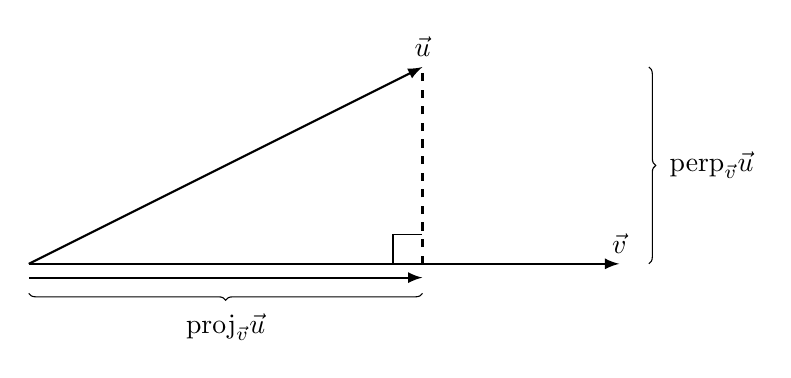
\begin{tikzpicture}[>=latex,scale=2.5]
		\draw[->,thick,black] (0,0) -- (2,1) node [above] {$\vec u$};
		\draw[->,thick,black] (0,0) -- (3,0) node [above] {$\vec v$};
		\draw[->,thick,black,yshift=-.07cm] (0,0) -- (2,0);
		\draw[decoration={brace, mirror}, decorate, yshift=-.15cm] (0,0) -- (2,0) node [midway,below,yshift=-4pt] {$\Proj_{\vec v}\vec u$};
		
		\draw[dashed,thick,black] (2,0) -- (2,1);
		\draw[decoration={brace, mirror}, decorate, xshift=1.15cm] (2,0) -- (2,1) node [midway,right,xshift=4pt] {$\Perp_{\vec v}\vec u$};
		\draw[thin,black] (1.85,0)--(1.85,.15)--(2,.15);

	\end{tikzpicture}
	\end{center}
	\vspace{-.6cm}
	
	The \emph{projection} of $\vec u$ onto $\vec v$ is written $\proj_{\vec v}\vec u$ and is the vector in the direction of $\vec v$
	such that $\vec u-\Proj_{\vec v}\vec u$ is orthogonal to $\vec v$.  The vector $\vec u-\Proj_{\vec v}$ is called the \emph{perpendicular
	component} of $\vec u$ with respect to $\vec v$ and is notated as $\Perp_{\vec v}\vec u$.
	\end{Def}
	
	\sep
	\vspace{-1cm}
	\begin{center}
	\usetikzlibrary{patterns,decorations.pathreplacing}
	\begin{tikzpicture}[>=latex,scale=2.5]
		\draw[->,thick,black] (0,0) -- (30:2) node [above] {$\vec a$};
		\draw[->,thick,black] (0,0) -- (3,0) node [above] {$\vec b$};
		\draw[thick,black] (0,0) +(0:.3cm) arc (0:30:.3cm) node[right,yshift=-4pt] {$\theta$};

	\end{tikzpicture}
	\end{center}

	In this picture $\|\vec a\|=4$, $\theta = \pi/6$, and $\vec b=\mat{6\\0}$.
	%%%
	% XXX: This is confusing with multiple b vectors. Should instead emphasise that proj_b(a ) = proj_{-b}(a).
	%%%
	\begin{Enum}
		\item   Write $\vec a$ in column vector form.
		\item   Find $\|\Proj_{\vec b}\vec a\|$ and $\|\Perp_{\vec b}\vec a\|$.
		\item Write down 
				$\Proj_{\vec b}\vec a$ and $\Perp_{\vec b}\vec a$ in column vector
				form.
		\item If $\vec c=\mat{-4\\0}$, write down 
				$\Proj_{\vec c}\vec a$ and $\Perp_{\vec c}\vec a$ in column vector
				form.
		\item If $\vec d=\mat{3\\1}$, write down 
				$\Proj_{\vec d}\vec a$ and $\Perp_{\vec d}\vec a$ in column vector
				form.  (You may need to use your knowledge of how dot products and angles
				relate to answer this one.)
		\item Consider $\vec d=\mat{3\\1}$.  Compute $\proj_{\xh}\vec d$ and 
		$\proj_{\yh}\vec d$.  How do these projections relate to the coordinates of $\vec d$? What
		can you say in general about projections onto $\xh$ and $\yh$?
	\end{Enum}
	
\newpage
\section*{Lines, Planes, Normals, and Equations}
	\sep
	\vspace{-1cm}
	\begin{Enum}
		\item Draw $\vec u=\begin{bmatrix}2\\3\end{bmatrix}$ and \emph{all}
		vectors perpendicular to it.
		\item If $\vec x=\begin{bmatrix}x\\y\end{bmatrix}$ and $\vec x$ is 
		perpendicular to $\vec u$, what is $\vec x\cdot \vec u$?
		\item Expand the dot product $\vec u\cdot \vec x$ to get an equation
		for a line.  This equation is called the \emph{scalar equation} representing the line.
	\end{Enum}

	\begin{Def}
		A \emph{normal vector} to a line (or plane or hyperplane) is a non-zero vector that is orthogonal to it.
	\end{Def}

	\begin{Enum}[resume]
		\item Rewrite the line $\vec u\cdot \vec x = 0$ in $y=mx+b$ form and verify it matches
		the line you drew above.
	\end{Enum}

	\sep
	We can also write a line in \emph{parametric form} by introducing a parameter
	that traces out the line as the parameter runs over all real numbers.
	\begin{Enum}
		\item Draw the line $L$ with $x,y$ coordinates given by
		\[
			\begin{array}{l}x=t\\y=2t\end{array}
		\]
		as $t$ ranges over $\R$.
		\item Write the line $\vec u \cdot \vec x=0$ (where $\vec u$ is the same as before) in parametric form.
	\end{Enum}
	
	\sep
	\emph{Vector form} is the same as parametric form but written in vector notation.  For example, the
	line $L$ from earlier could be written as 
	\[
		\begin{bmatrix}x\\y\end{bmatrix}=\begin{bmatrix}t\\2t\end{bmatrix}
	\]
	or
	\[
		\begin{bmatrix}x\\y\end{bmatrix}=t\begin{bmatrix}1\\2\end{bmatrix}.
	\]

	\begin{Enum}
		\item Write the line $\vec u\cdot \vec x=0$ in vector form.  That is, find a vector $\vec v$ so
		the line $\vec u\cdot \vec x=0$  can be written as
		\[
			\begin{bmatrix}x\\y\end{bmatrix} = t\vec v
		\]
		as $t$ ranges over $\R$.
		\item What is $\vec v\cdot \vec u$? Why? Will this always happen?
	\end{Enum}

\newpage

	\subsection*{Moving to Planes}
	
	\sep
	\vspace{-1cm}
	\begin{Enum}
		\item Write down three solutions $\vec a$, $\vec b$, $\vec c\in\R^3$ to
		\begin{equation}\label{eq1}
			2x+y-z=0.
		\end{equation}
		\item Find $\vec n\in\R^3$ so that equation (\ref{eq1}) is equivalent
		to $\vec n\cdot \vec x=0$ where $\vec x=\begin{bmatrix}x\\ y\\ z\end{bmatrix}$.
		\item What do you notice about the angle between solutions to equation (\ref{eq1}) and $\vec n$?
	\end{Enum}

	When writing down solutions to equation (\ref{eq1}), you got to choose two coordinates before the remaining
	coordinate became determined.  This means the solutions have two parameters (and consequently form a
	two dimensional space).

	\begin{Enum}[resume]
		\item Write down parametric form of a line of solutions to equation (\ref{eq1}).
		\item Write down parametric form of a different line of solutions to equation (\ref{eq1}).
		\item Write down all solutions to equation (\ref{eq1}) in parametric form.  That is, find $a_x,
		a_y,a_z,b_x,b_y,b_z$ so that
		\[
			\begin{array}{l}
				x=a_x t+b_x s\\
				y=a_y t+b_y s\\
				z=a_z t+b_z s
			\end{array}
		\]
		gives all solutions as $t,s$ vary over all of $\R$.
		\item Write all solutions to equation (\ref{eq1}) in vector form.
	\end{Enum}

\subsection*{Arbitrary Lines and Planes}
	
	So far, all of our lines and planes have passed through the origin. To 
	produce the equation of an arbitrary line/plane, we first make one of
	same ``slope'' that passes through the origin, then we translate it
	to the appropriate place.

	\sep
	We'd like to write the equation of a line $L$ with normal vector
	$\vec n=\begin{bmatrix}4\\-1\end{bmatrix}$ that passes through
	the point $p=\mat{-1\\-1}$

	\begin{Enum}
		\item Give a scalar equation of the line $L_2$ which is parallel to $L$
		but passes through the origin.
		\item Draw a picture of $L$ and $L_2$, and find two points that lie on
		$L$.  Call these points $p_1$ and $p_2$.
		\item Verify the vector $\overline {p_1p_2}$ is orthogonal to $\vec n$.
		\item What is $\vec n\cdot p_1$, $\vec n\cdot p_2$, $\vec n\cdot p$?
		Should these values be zero, equal, or different?  Explain (think about
		projections).
		\item How does the equation $\vec n\cdot (\vec x-p)=0$ relate to $L$?
	\end{Enum}

	\sep
	$W$ is the plane with normal vector $\vec n=\mat{1\\2\\3}$ and that passes through
	the point $p=\mat{1\\1\\2}$.
	\begin{Enum}
		\item Write normal form of $W$.
		\item Write vector form of $W$.
	\end{Enum}

\newpage

\section*{Arc Length}

	\sep
	The parameterized curve
	\[
		\vec r(t) = \mat{2\cos t\\2\sin t}
	\]
	describes the position of a particle at time $t$.
	\begin{Enum}
		\item Describe the path and motion of this particle in words.
		\item Compute the displacement  of the particle between $t=0$
			and $t=\Delta t$ and call the resulting vector $\Delta \vec r$.  
			(Assume $\Delta t$ is small.)
		\item Approximate the length of $\Delta \vec r$.  You may use the fact that
			\[
				\sin x\approx x\qquad\text{and}\qquad \cos x\approx -\tfrac{1}{2}x^2+1
			\]
			when $x\approx 0$.
		\item Use a limit to compute the velocity of the particle at $t=0$. Call this 
			vector $\vec v_0$.
		\item Use a limit to compute the speed at $t=0$.  Call this value $s_0$.
		\item How do $\|\vec v_0\|$ and $s_0$ relate?  Why?
	\end{Enum}

	\sep
	A particle's path is parameterized by
	\[
		\vec m(t) = (f(t), g(t), h(t))
	\]
	where $t$ represents time.
	\begin{Enum}
		\item Derive (with explanation) a formula for the velocity of
			the particle at time $t=t_0$.
		\item Derive (with explanation) a formula for the speed of
			the particle at time $t=t_0$.
	\end{Enum}
	
	\sep
	Recall the particle whose path is given by
	$
		\vec r(t) = \mat{2\cos t\\2\sin t}
	$
	where $t$ represents time.
	\begin{Enum}
		\item Use the fact that
			\[
				\text{distance traveled}=\int\text{\it speed}\ \mathrm{d}\text{\it time}
			\]
		to produce a formula for how far the particle has traveled from $t=0$ to $t=t_0$.
		\item Use geometry to do the same thing.
		\item Derive an expression (with explanation) for the arc length of $\vec m(t) = (f(t), g(t), h(t))$
			from $t=0$ to $t=t_0$.
	\end{Enum}

\subsection*{Arc Length Parameterization}
	
	An \emph{arc length parameterization} of a curve $C$ is a function $\vec s:\R\to\R^n$ whose
	image is $C$ with the added property that the arc length of $\vec s(t)$ from $t=0$ to $t=t_0$
	is $t_0$ for all valid choices of $t_0$.  I.e., the distance traveled by the parameter along
	$\R$ is the same as the distance traveled by the point $\vec s(t)$ in $\R^n$.

	\sep
	\vspace{-1cm}
	\begin{Enum}
		\item Produce an arc length parameterization of the curve parameterized by
			$
				\vec r(t) =\mat{2\cos t\\ 2\sin t}.
			$
		\item Produce an arc length parameterization of the curve parameterized by
			$
				\vec q(t) =\mat{t\\ t^{3/2}}.
			$
	\end{Enum}

	
	An arc length parameterization of a curve can also be thought of
	as a parameterization where a particle always moves at unit speed 
	(if you interpret a parameterized curve as describing the motion of a
	particle).

	By reparameterizing, we can describe the motion of a particle along
	a path at any speed.

	\sep
	A particle moves along a path $C$, which is a circle in $\R^2$ of radius $3$, centered at the origin, and oriented counter-clockwise.
	\begin{Enum}
		\item Parameterize $C$ so that the speed is $2.5$.
		\item Parameterize $C$ so that the speed of the particle starts and ends at $0$.
		\item Parameterize $C$ so that the speed of the particle starts at $0$ and ends at $4$.
		\item Parameterize $C$ so that the speed of the particle is $0$ at six points along the curve.
	\end{Enum}

	\sep
	A particle's motion is described by the function $\vec h(t) = \mat{f(t)\\ g(t)}$,  which is a 
	parameterization of the curve $H$.  The arc length of $H$ from $t=0$ to
	$t=t_0$ using this parameterization is is given by the function $s(t_0) = t_0^2$.
	\begin{Enum}
		\item Write an expression for the speed of the particle at time $t$.
		\item Give a formula for the arc length parameterization of $H$.
	\end{Enum}

	
\section*{Tangents, Normals, and Acceleration}
	
	\vspace{-1cm}
	\begin{Def}
	Suppose $\vec r(t)$ describes the motion of a particle.  The \emph{velocity}
	of the particle is defined as
	\[
		\vec v(t) = \lim_{h\to 0} \frac{\vec r(t+h)-\vec r(t)}{h}.
	\]
	The \emph{acceleration}
	of the particle is defined as
	\[
		\vec a(t) = \lim_{h\to 0} \frac{\vec v(t+h)-\vec v(t)}{h}.
	\]
	\end{Def}
	Both $\vec v$ and $\vec a$ are vector-valued derivatives.

	\sep
	Let $\vec r(t) = \mat{t+2\\ \sin t\\ t^3}$ represent the position of a particle at time $t$.
	\begin{Enum}
		\item Find the velocity of the particle at time $t$.
		\item Find the acceleration of the particle at time $t$.
	\end{Enum}

	\sep
	Let $\vec r_\ell(t) = \mat{\frac{t^2}{2}\\\frac{t^2}{2}}$ and $\vec r_c(t) = \mat{\cos t\\ \sin t}$ represent the position
	of the particles $r_\ell$ and $r_c$ at time $t$.
	\begin{Enum}
		\item Describe the paths of each of these particles.  What should their accelerations be?  Why?
		\item Compute the accelerations of $r_\ell$ and $r_c$ at time $t$.
		\item Compute the tangent vectors for the functions $\vec r_\ell$ and $\vec r_c$ at time $t$.
			How does the direction of the tangent vectors and the direction of the acceleration vectors
			compare?
	\end{Enum}

	If $\vec r(t)$ describes the position of a particle at time $t$ and $\vec a(t)$ its acceleration, $\vec a(t)$
	can be decomposed into a \emph{tangential} component, $\vec a_T(t)$, and a \emph{normal} component $\vec a_N(t)$
	so that
	\[
		\vec a(t) = \vec a_T(t) +\vec a_N(t).
	\]

	\sep
	Let $\vec r_{c\ell}(t) = \mat{\frac{t^2}{2}+\cos t\\\frac{t^2}{2}+\sin t}$  represent the position
	of the particle $r_{c\ell}$ at time $t$.
	\begin{Enum}
		\item Compute the tangential and normal components of the acceleration of $r_{c\ell}$.
		\item By changing the speed of $r_{c\ell}$ (but not its path), is it possible to make 
			the tangential component of its acceleration zero?
		\item By changing the speed of $r_{c\ell}$ (but not its path), is it possible to make 
			the normal component of its acceleration zero?
	\end{Enum}

	We're going to develop some tools to mathematically verify our intuition about the acceleration
	vector.

	\sep
	\vspace{-1cm}
	\begin{Enum}
		\item Suppose $\vec p(t)$ and $\vec q(t)$ are both vector-valued functions.  Expand $\vec p(t)\cdot\vec q(t)$
		using components. Now, come up with an expression for $\Big(\vec p(t)\cdot\vec q(t)\Big)'$.  Look at your
		result and rewrite it as an expression involving dot products.
		You've just discovered a product rule for the dot product!
		\item Using similar methods to the computation of $\Big(\vec p(t)\cdot\vec q(t)\Big)'$, find an expression
			for $\|\vec p(t)\|'$.
		\item If a particle whose path is given by $\vec r(t)$ is moving at unit speed, then $\|\vec v(t)\| = 1$.
			Take derivatives of both sides of this expression to show that $\vec v(t)\cdot \vec a(t) = 0$.
	\end{Enum}

%
%	\vspace{-.7cm}
%	\begin{Def}
%		Suppose $\vec r_s(t)$ is an arc length parameterization of some curve $C$.
%		The \emph{curvature} of $C$ at the point $\vec r_s(t)$ is
%		\[
%			\kappa(t) = \|\vec a_s(t)\|
%		\]
%		where $\vec a_s(t)$ is the second derivative of $\vec r_s(t)$.
%	\end{Def}
%
%	Having an arc length parameterization of $C$ is essential in order to use this definition
%	of curvature, but when computing curvature, we can do without.
%
%	\sep
%	Let 
%	\begin{Enum}
%		\item 
%	\end{Enum}


\vspace{-.5cm}
\section*{Visualizing Surfaces}
	As we've already seen, being able to picture multi-dimensional objects is 
	invaluable when intuiting solutions and when coming up with mathematical
	justifications for intuition.  There are two main ways we visualize
	2D surfaces: perspective drawings and level-curves.


	\sep
		Consider the surface defined by $z=f(x,y)$ where $f(x,y)=x^2+y^2$.
	\begin{Enum}
		\item On a single $xy$-plane, draw the set of points satisfying the equations $0=f(x,y)$, $1=f(x,y)$,
			$2=f(x,y)$, $3=f(x,y)$, and $4=f(x,y)$.  What is the set of points satisfying $-1=f(x,y)$?
	\end{Enum}
	The curves you just drew are called \emph{level curves}.
	\begin{Enum}[resume]
		\item Plot in 3D the function $z=f(x,y)$ for $z=0,1,2,3,4$.  Are you able to see what this surface looks like?
		\item We can plot more and more contours of this surface until we have a good idea of what it looks like.
			Add the set of points $z=f(0,y)$ and $z=f(x,0)$ to your plot.
	\end{Enum}


	\sep
	Level curves are contours produced by fixing $z$ and graphing the result.  Other useful contours
	come about by fixing $x$ or $y$.  Use any contour-based method to plot the following surfaces.
	\begin{Enum}
		\item $z=x^2-y^2$
		\item $z^2=4x^2+y^2$
		\item $z^2=9-(4x^2+y^2)$
		\item $z=(\sin x)(\sin y)$
	\end{Enum}

\newpage
\section*{Directional Derivatives}

	\sep
	It is winter in Chicago.  Imagine a bug crawling along the floor of
	a room that is $7\times 7$ meters.  Figure \ref{heatcontour1} shows the contour plot of the heat
	of the floor in Fahrenheit.\footnote{The bug questions are due to Mairead Greene, Amy Ksir, and Christine von Renesse.}
	\begin{figure}[h!]
		\begin{center}
			\includegraphics[width=3.5in]{heat_contour1.pdf}
		\end{center}
		\vspace{-.5cm}
		\caption{Heat contours for a room.}
		\label{heatcontour1}
	\end{figure}
	\begin{Enum}
		\item Where is the door to the outside?  Where is the window?  Where is the heater? Why?
			What might be in the lower right corner of the room?
		\item The bug would like to crawl from the window to the right wall along a path that minimizes
			the change in temperature.  Draw two such paths.
		\item The bug makes a circuit around the entire room by walking along the walls clockwise.
			Draw a graph of distance verses temperature for this part of the bug's journey.  How
			do the starting values and ending values of your graph compare?  Is the accuracy of your
			graph limited?
	\end{Enum}
	
	\sep Figure \ref{heatcontour2} shows the path the bug decided to follow.
	\begin{figure}[h!]
		\begin{center}
			\includegraphics[width=3.5in]{heat_contour2.pdf}
		\end{center}
		\vspace{-.5cm}
		\caption{Heat contours for a room.}
		\label{heatcontour2}
	\end{figure}
	\begin{Enum}
		\item Find the average change in temperature from $P$ to $Q$ for the bugs journey.
		\item Estimate the instantaneous rate of change of temperature at the point $P$.
		\item Suppose $T(x,y)$ gives the temperature of the room at the coordinates $(x,y)$.
			Write a limit expression to compute the exact rate of change of temperature
			at the beginning of the bug's journey. Does the rate of change depend on time?
		\item Write a limit expression to compute the rate of change of temperature
			\emph{with respect to distance} at the start of the bug's journey.
		\item If the bug had decided to travel in a different direction, would the rate of change
			of temperature be the same?  Explain.
	\end{Enum}
	
	\newpage
	\sep
	Let $f(x,y) = 2(x-3)^2+y$
	\begin{Enum}
		\item Calculate the rate of change of $f$ at the origin 
			in the directions $\xh$, $\yh$, $\vec a=(\tfrac{\sqrt{2}}{2},\tfrac{\sqrt{2}}{2})$.
		\item Calculate the rate of change of $f$ at $p=(1,-1)$
			in the directions $\xh$, $\yh$, $\vec a=(\tfrac{\sqrt{2}}{2},\tfrac{\sqrt{2}}{2})$.
	\end{Enum}

\subsection*{A New Perspective on Derivatives}

	In single-variable calculus, we deal with functions $g:\R\to\R$.  The derivative of this function
	at a point $a$ is the rate of change of $g$ at the point $a$.

	\sep
	Let $g(x)=x^2$.
	\begin{Enum}
		\item What is the rate of change of $g$ at the points $x=0,1,$ and $2$?  How about at $x=x_0$?
		\item Use your knowledge of the rate of change of $g$ to \emph{approximate} $g(x)$ where
			$x=0+\varepsilon, 1+\varepsilon,$ and $2-\varepsilon$ where $\varepsilon>0$ is a tiny number.
		\item Write down three functions: $G_0$, $G_1$, and $G_2$ so that if $\varepsilon$ is tiny, $g(a+\varepsilon)\approx
			g(a) + G_a(\varepsilon)$.  
	\end{Enum}

	\sep
	Recall $f(x,y)=2(x-3)^2+y$ from before.
	\begin{Enum}
		\item Write down a function $F_{(0,0)}:\R^2\to\R$ such that if $\vec u$ is a vector
			and $\|\vec u\|$ is tiny, 
			\[
				f(\vec 0+\vec u)\approx f(\vec 0) + F_{(0,0)}(\vec u).
			\]
			Notice, $F_{(0,0)}$ is somehow representative of the rate of change of $f$ at $(0,0)$.
			It may help to compute $F_{(0,0)}$ for several example directions before coming up
			with a formula.
		\item Write down a function $F_{(1,-1)}$ so that if $\vec u$ is a vector and $\|\vec u\|$ is
			tiny, $f\Big((1,-1)+\vec u\Big)\approx f(1,-1)+F_{(1,-1)}(\vec u)$.
		\item Can a single number represent the rate of change of $f$ at the point $(0,0)$?  Why or why not?
			If a number cannot, can you think of another object that can?
	\end{Enum}

\newpage

	\begin{Def}
		The \emph{directional derivative} of a function $f:\R^n\to\R^m$ at the
		point $\vec a$ in the direction $\vec u$ is
		\[
			D_{\vec a}f(\vec u) = \lim_{h\to 0} \frac{f(\vec a+h\vec u)-f(\vec a)}{h}.
		\]
		I.e., it is the rate of change of $f$ at $\vec a$ heading in the direction of $\vec u$
		with speed $\|\vec u\|$.
	\end{Def}

	\sep
	Let $f(x,y) = (x+1)^2+2y$.
	\begin{Enum}
		\item Give a parameterization of all two dimensional unit vectors.
		\item Use the definition of the directional derivative to compute
			the directional derivative of $f$ at the point $(0,0)$ in the
			direction of each of your parameterized unit vectors.
		\item Find the direction of the maximal directional derivative.  You
			may find the identity $\sin t+\cos t = \sqrt{2}\sin(t+\tfrac{\pi}{4})$
			helpful.
	\end{Enum}

	\vspace{-.7cm}
	\begin{Def}
		The \emph{gradient} of a function $f:\R^n\to \R$ is
		\[
			\nabla f  = \left(
				\frac{\partial f}{\partial x_1}, 
				\frac{\partial f}{\partial x_2}, \ldots,
				\frac{\partial f}{\partial x_n}
			\right)
		\]
		where $x_1,\ldots, x_n$ are the parameters of $f$.
	\end{Def}
	
	\sep
	Let $f(x,y) = (x+1)^2+2y$ as before.
	\begin{Enum}
		\item Compute $\nabla f(0,0)$ (the gradient of $f$ at the point $(0,0)$).
		\item Compute $\nabla f(0,0)\cdot \vec u$ for each of your parameterized unit vectors $\vec u$.
			What do you notice?
		\item Make a conjecture about how the gradient of a function can be used to compute directional derivatives.
	\end{Enum}

	\sep
	Sticking with $f(x,y) = (x+1)^2+2y$, consider the surface $S=\{\big(x,y,f(x,y)\big):x,y\in\R^2\}$.
	\begin{Enum}
		\item Describe $S$.  If $a\in S$, what should \emph{the tangent plane to $S$ at $a$} mean?
		\item Compute the tangent plane, $\mathcal P$, to $S$ at the point $\big(0,0,f(0,0)\big)$ in vector form.
		\item Find standard/normal form of the tangent plane and solve for $z$.  That is,
			find an equation for the tangent plane in the form $z=ax+by+c$.  Do the values $a$, $b$, and
			$c$ look familiar?
		\item Consider the function $g=f-\mathcal P$.  That is, $g(x,y)=f(x,y)-z(x,y)$ where $z(x,y)$ is the
			equation of the tangent plane.  What should the directional derivative of $g$ at $(0,0)$ be?
			Does it depend on direction?
	\end{Enum}

	So far, the gradient has been appearing in directional derivatives and tangent planes.
	One might even argue that the gradient \emph{is} the derivative.  Unfortunately, the gradient
	of a function existing is not sufficient for a function to be differentiable.

	\vspace{-.7cm}
	\begin{Def}
		The function $f:\R^n\to \R$ is \emph{differentiable} at $\vec a=(a_1,\ldots,a_n)$ if there exists
		a tangent plane at $\vec a$.  That is, there exists some function $p(x_1,\ldots, x_n)
		= c+\sum \alpha_i (x_i-a_i) = c+\vec \alpha \cdot(\vec x-\vec a)$ so that
		\[
			\lim_{\|\vec u\|\to0} \frac{f(\vec a + \vec u)-p(\vec a + \vec u)}{\|\vec u\|} = 0.
		\]
	\end{Def}

	There's just one trouble with this definition.  How do we take a limit as $\|\vec u\|\to 0$?

\newpage
\subsection*{Multidimensional Limits}

	\begin{Def}
		If $f:\R^n\to \R$, then the \emph{limit of $f$ at $\vec a$} exists and is equal to $L$, written
		$\displaystyle \lim_{\vec x\to\vec a} f(\vec x) = L$, if
		for all $\varepsilon > 0$ there exists a $\delta > 0$ such that
		\[
			0<\|\vec x-\vec a\| <\delta \qquad \text{implies}\qquad |f(\vec x) - L| < \varepsilon.
		\]
		If no such $L$ exists, we say the limit does not exist.
	\end{Def}
	When first considered, the definition of limit can be confusing, so let's play with some functions
	that we're familiar with.

	\sep
	Let $f(x) = 3x$.
	\begin{Enum}
		\item  Draw the graph of $f$ and use your intuition to guess $\lim_{x\to 0} f(x)$.  Call your
			guess $L$.
		\item If $\varepsilon = 1/2$, can you find a $\delta$ so that if $|x-0|<\delta$ we can be assured
			$|f(x)-L|<\varepsilon$?
		\item If $\varepsilon = 1/4$, can you find a $\delta$ so that if $|x-0|<\delta$ we can be assured
			$|f(x)-L|<\varepsilon$?
		\item Come up with a rule for how to choose an appropriate $\delta$ for any $\varepsilon$.
	\end{Enum}

	\sep
	Let $g(x) = \frac{x}{|x|}$, and let $L$ be a guess for $\lim_{x\to 0} \frac{x}{|x|}$.
	\begin{Enum}
		\item Suppose we guess $L=1$.  Picking $\varepsilon = 3/2$, can you find an appropriate
			$\delta$?  What if $L=-1$?  For $\varepsilon=3/2$, can you find an appropriate $\delta$?
			What if $L=0$?  What values can we rule out as possibilities for $L$?
		\item Suppose we guess $L=0$.  Picking $\varepsilon=3/2$, can you find an appropriate $\delta$?
			Is $0$ the limit?  Explain.
		\item Find an $\varepsilon$ that shows that $g$ has no limit at $0$.
	\end{Enum}

	\sep
	Let $h(x,y) = \frac{xy^2}{x^2+y^2}$.
	\begin{Enum}
		\item Give a parameterization of all vectors in $\R^2$ with length $r$.
		\item If $\vec u\in \R^2$ satisfies $\|\vec u\|=r$, can you give upper
			and lower bounds on $h(\vec u)$?
		\item Explain why the limit $\displaystyle \lim_{\|\vec u\|\to 0} h(\vec u)$
			does or doesn't exist.
	\end{Enum}
	\sep
	Let $h(x,y) = \frac{xy}{x^2+y^2}$.
	\begin{Enum}
		\item Give a parameterization of all vectors in $\R^2$ with length $r$.
		\item If $\vec u\in \R^2$ satisfies $\|\vec u\|=r$, can you give upper
			and lower bounds on $h(\vec u)$?
		\item Explain why the limit $\displaystyle \lim_{\|\vec u\|\to 0} h(\vec u)$
			does or doesn't exist.
	\end{Enum}


\newpage
\subsection*{Lagrange Multipliers}

	\sep
	We know that $\nabla f(\vec a)\cdot \vec u$ gives the directional derivative
	of $f$ at the point $\vec a$ in the direction $\vec u$.  Suppose
	$\nabla f(\vec a) = (1,3)$.
	\begin{Enum}
		\item What is the direction of the biggest rate of change of $f$ at $\vec a$? Why?
		\item In what direction is the least change in $f$ at $\vec a$?
	\end{Enum}

	\sep
	Suppose $C$ is a level curve of $f$.  For $\vec a\in C$, suppose $\vec T_a$ is a tangent vector to
	$C$ at $\vec a$.
	\begin{Enum}
		\item What is the rate of change of the function $f$ at $\vec a$ in the direction $\vec T_a$?
		\item What is $\nabla f(\vec a)\cdot \vec T_a$?
		\item If $f(x,y)=x^3+y^2$, find a tangent vector to the curve $C=\{(x,y):f(x,y)=2\}$ at $(1,1)$.
	\end{Enum}

	\sep
	Consider a function $f:\R^2\to \R$ and a curve $C$ (not a level curve).  Let $\vec r(t)$
	be a parameterization of $C$.  We are interested in the minimum and maximum values for 
	$f\circ \vec r$ (i.e., the min/max values of $f$ on the curve $C$).
	\begin{Enum}
		\item What will $(f\circ \vec r)'$ be at a local maximum or minimum?
		\item Explain how to interpret the quantity $(f\circ \vec r)'(t)$
			as a directional derivative.
		\item Use your knowledge of how the gradient allows you to compute directional derivatives
			to come up with a ``chain rule'' for the expression $(f\circ \vec r)'(t)$.
		\item Suppose $f(x,y) = 2x+y$ and $C$ is a circle of radius 1 centered at $\vec 0$.
			Parameterize $C$ and attempt to find the maximum value that $f$ takes on the curve $C$.
			Are these computations easy?
	\end{Enum}

	\sep
	Let $f(x,y)=2x+y$ and let $C$ be a circle of radius 1 centered at $\vec 0$.
	\begin{Enum}
		\item Find a function $g:\R^2\to \R$ so that $C$ is a level curve of $g$.
			Can you pick $g$ so that $C=\{(x,y): g(x,y)=0\}$?
		\item What is the relationship between a tangent vector to $C$ at $\vec a$ and
			$\nabla g(\vec a)$?
		\item Suppose that on the curve $C$, $f$ attains 
			a maximum at $\vec a\in C$. What then is the relationship between 
			$\nabla f(\vec a)$ and $\nabla g(\vec a)$?  Can you describe this relationship
			with a formula?
		\item Use your formula from the previous part along with the constraint $g(x,y)=0$
			to find the maximum value the function $f$ attains on the curve $C$.  Congratulations,
			you've just discovered \emph{Lagrange Multipliers}!

	\end{Enum}

	\sep
	We will use Lagrange Multipliers to find the dimensions of the largest box (the one with the most volume)
	given that the surface area is $32$.
	\begin{Enum}
		\item Write down the function we wish to optimize, call it $f$, and rephrase our constraint
			on surface area so that we may interpret it as the level curve of some function $g$.
		\item Write down a relationship between $\nabla f$ and $\nabla g$ at the maximum.
		\item Write down all equations obtained thus far, and attempt to solve for the dimensions of the box.
			Do we need to solve for every variable?
	\end{Enum}
\newpage

\section*{Iterated Integrals}
	Integrals add things up, and iterated integrals are no different; it's just that instead of adding things
	up in one dimension, we add things up in multiple dimensions.

	\sep
	To get our bearings, let's revisit integrating with respect of $\mathrm{d}x$ and $\mathrm{d}y$
	when finding area.  Let $T$ be the triangle with vertices $(0,0)$, $(4,0)$, and $(4,3)$.
	\begin{Enum}
		\item Draw a picture representing how a Riemann sum could be used to compute the area of $T$.
		\item Draw a picture representing a different way to compute the area of $T$ using a Riemann sum.
		\item Compute the area of $T$ using an integral with respect to $x$; now using an integral with 
			respect to $y$; now using the formula $\frac{1}{2}base\times height$.
	\end{Enum}

	\sep
	Let $T$ be the triangle with vertices $(0,0)$, $(4,0)$, and $(4,3)$, and imagine that $T$
	outlines a triangular strip of foil.  The density of this foil at any given point (in the 
	first quadrant) is
	$\rho(x,y) = x^2+y$.
	\begin{Enum}
		\item Using the fact that for this foil, $mass=density\times area$, write down two different
			integrals that would compute the total mass of $T$, and draw their corresponding
			Riemann-sum pictures.
		\item Evaluate your two integrals.  Is one easier to evaluate than the other?
		\item Can $(x^2+y)\mathrm{d}x\mathrm{d}y$ be interpreted on its own?
	\end{Enum}

	\sep
	Let the region $R\subset \R^2$ be the area between the parabola $x=y^2$ and the line $x=1$.  Let 
	$f(x,y)=3x+y^2$.
	\begin{Enum}
		\item Write down two different iterated integrals to compute $\displaystyle \iint_R f(x,y)\d x\d y$.
		\item Is one of your integrals easier to evaluate than the other?
		\item Describe and draw a region $A$ so that 
			$\displaystyle\iint_A f(x,y)\d x\d y = \int_{x=0}^{x=1}\int_{y=-\sqrt{1-x^2}}^{y=\sqrt{1-x^2}} f(x,y)\d y\d x$.
	\end{Enum}

\subsection*{The Volume Form}
	We've been using integrals to find the area or volume (or hypervolume) under a curve.
	Abstractly, this process has been the same every time: chop the region into little pieces, and
	add up each piece's contribution with an integral to find the total.  We're continuing the same
	process, but we're going to start chopping regions up into (sometimes) non-rectangular chunks.

	\sepl
	\begin{Enum}
		\item Draw the lines $x=x_0$, $x=x_0+\Delta x$, $y=y_0$ and $y=y_0+\Delta y$ where
			$\Delta x$ and $\Delta y$ are assume to be small.  Write down a formula for the area enclosed by
			those lines.  Does your formula depend on $x_0$ and $y_0$?
		\item Draw the curves, specified in polar coordinates by $r=r_0$, $r=r_0+\Delta r$, $\theta = \theta_0$,
			and $\theta = \theta_0+\Delta\theta$ where $\Delta r$ and $\Delta \theta$ are assumed to
			be small.  Write down a formula for the area enclosed by those curves.  Does your
			formula depend on $r_0$ and $\theta_0$?
		\item Using the idea that a limit as $\Delta ?\to 0$ of a Riemann sum results in an integral, 
			write down a double-integral expression for the area of a semicircle of radius $1$
			in both rectangular and polar coordinates.
		\item Let $V(r_0,\theta_0) = r_0\Delta r\Delta\theta$, and let $\Delta V(r_0,\theta_0)$ be the exact
			area of the annular (ring-shaped) section you found earlier.  What is $\displaystyle \lim_{\Delta r, \Delta\theta\to 0}
			\frac{\Delta V(r_0,\theta_0)}{V(r_0,\theta_0)}$?  Do we need the $(\Delta r)^2\Delta \theta$ term
			at infinitesimal scales?
	\end{Enum}

	\begin{Def}
		Suppose $\mathcal F$ is a coordinate system for $\R^2$ with a relationship
		to rectangular coordinates given by 
		$x=f_1(a,b)$ and $y=f_2(a,b)$.  The \emph{pre-volume form} associated with $\mathcal F$
		at the point $(a,b)$ is written $\Delta V(a,b)$ and is the area between the curves
		$a=a_0$, $a=a_0+\Delta a$, $b=b_0$, and $b=b_0+\Delta b$.

		The \emph{volume form} associated with $\mathcal F$ at $(a,b)$ is the infinitesimal 
		$\d V(a,b)=V(a,b)\d a\d b$ where $V$ is the unique function satisfying
		\[
			\lim_{\Delta a,\Delta b\to 0} \frac{\Delta V(a,b)}{V(a,b)\Delta a\Delta b} = 1
		\]
		and can obtained by replacing $\Delta w$ with $\d w$ and $(\Delta w)^2$ with $0$ in
		the pre-volume form (where $w$ stands for any variable).
	\end{Def}
	For coordinate systems in $\R^3$ (and $\R^n$), the volume form is defined in an analogous way.


	\sepl
	\begin{Enum}
		\item Write down the pre-volume and volume forms for polar coordinates.  What are the functions
			$f_1$ and $f_2$ for polar coordinates?
		\item Write down the pre-volume and volume forms for rectangular coordinates.  What
			are the functions $f_1$ and $f_2$?
		\item Let $\mathcal S$ be a stretched coordinate system.  That is, the point $(a,b)$ in
			$\mathcal S$-coordinates corresponds to the point $(a/2, b/3)$ in rectangular 
			coordinates.  Write down the pre-volume and volume forms for $\mathcal S$-coordinates.
		\item Consider the set $X=\{(a,b): 0\leq b\leq a^2\text{ and }0\leq a\leq 1\}$ specified in $\mathcal S$ coordinates.
			Draw $X$ on the $\mathcal S$-coordinate plane and in standard coordinate plane.  Then, compute
			the area of $X$ by setting up an integral using the volume form for $\mathcal S$ coordinates.
	\end{Enum}

	\sep
	Let $f(x,y)=x^2+y^2$ and let $D$ be a disk of radius 2 centered at the origin.  We would like to
	find $A=\displaystyle \int_D f\d V$.
	\begin{Enum}
		\item Write down the bounds of $D$ in rectangular coordinates and set up (but don't evaluate)
			an integral for $A$.
		\item Write down the bounds of $D$ in polar coordinates and set up (but don't evaluate) an 
			an integral for $A$.
		\item Find $A$ by evaluating whichever integral you want.
	\end{Enum}

	\sep
	Cylindrical coordinates for $\R^3$ take the form $(r,\theta, z)$ where the
	$xy$-plane is specified in polar coordinates by the first two components
	and the height along the $z$-axis
	is given by the third component.
	\begin{Enum}
		\item Compute the volume form for cylindrical coordinates.
		\item A discuss is constructed from gluing two cones' bases together.
			The radius of the base of each cone is $4$ and the height of each
			cone is $1$.  Describe the surface of the discuss using cylindrical coordinates
			(you may need to describe the top and bottom separately)
		\item The discuss has a density given by $\rho(x,y,z) = x^2+y^2+2|z|$.  Find the
			mass of the discuss. (You may exploit symmetry.)
	\end{Enum}


%\begin{tikzpicture}
%	\begin{axis}[view/az=14]
%	\addplot3[mesh,draw=red,samples=10] {x^2-y^2};	
%	\end{axis}
%\end{tikzpicture}
%
%
%
%\begin{tikzpicture} 
%\begin{axis}[ title={$x \exp(-x^2-y^2)$ and its gradient}, domain=-2:2, view={0}{90}, axis background/.style={fill=white}, ] 
%	\addplot3[blue, quiver={ u={exp(0-x^2-y^2)*(1-2*x^2)}, v={exp(0-x^2-y^2)*(-2*x*y)}, scale arrows=0.3, }, -stealth,samples=15] {exp(0-x^2-y^2)*x}; 
%\end{axis} 
%\end{tikzpicture}

	
	
\newpage

$\phantom{x}$
\newpage
\section*{Systems of Linear Equations}
	
	\emph{Linear equations} are equations only involving variables, 
	multiplication by constants, and addition/subtraction.  \emph{Systems}
	of equations are sets of equations that share common variables.

	\sep
	Consider the system
	\begin{equation}\label{eq2}
		\begin{array}{ll}
			x-y &= 2\\
			2x+y &= 1
		\end{array}
	\end{equation}

	\begin{Enum}
		\item Draw the lines in (\ref{eq2}) on the same coordinate plane.
		\item Algebraically solve the system (\ref{eq2}).  What does this 
		solution represent on your graph?
	\end{Enum}
	
	\sep
	Let $L$ be the line given by $x-y=2$.
	\begin{Enum}
		\item Write an equation of a line that doesn't intersect $L$.
		\item Write an equation of a line that intersects $L$ in 
		\begin{enumerate}
			\item one place.
			\item infinitely many places
			\item exactly two places
		\end{enumerate}
		or explain why no such equation exists.
		\item For each equation you came up with, solve the system algebraically.
		How can you tell algebraically how many solutions there are?
	\end{Enum}

\subsection*{The Row Reduction Algorithm}

	\sep
	\vspace{-1cm}
	\begin{Enum}
		\item Solve the system
		\begin{equation}\label{eq3}
			\begin{array}{ll}
				x-y-2z &= -5\\
				2x+3y+z &= 5\\
				0x+2y+3z &= 8
			\end{array}
		\end{equation}
		any way you like.

		\item Use an augmented matrix to solve the system (\ref{eq3}).
	\end{Enum}

	The system (\ref{eq3}) can be interpreted in two ways (and switching between these 
	interpretations when appropriate is one of the most powerful tools of Linear 
	Algebra).  We can think of solutions to (\ref{eq3})
	as the intersection of three planes, or we can interpret the solution
	as coefficients of a linear combination.

	\begin{Enum}[resume]
		\item Rewrite (\ref{eq3}) as a vector equation of the form
		\[
			x\vec v_1+y\vec v_2+z\vec v_3 = \vec p
		\]
		where $x,y,z$ are interpreted as scalar quantities.

		\item If $(x,y,z)$ is a solution to (\ref{eq3}), explain how to get from the
		origin to $\vec p$ using only $\vec v_1, \vec v_2, \vec v_3$.
		\item If $(x,y,z)$ is a solution to \eqref{eq3}, is $\vec p\in\Span\{\vec v_1,\vec v_2,\vec v_3\}$?
	\end{Enum}

	\sep
	Consider the augmented matrix
	\[
		A=\left[\begin{array}{ccc|c}
			1 & 2 & -1 & -7\\
			0 & 2 & 3 & 9\\
			0 & 0 & 1 & 1
		\end{array}\right].
	\]
	\begin{Enum}
		\item Write the system of equations corresponding to $A$.
		\item Solve the system of equations corresponding to $A$.
	\end{Enum}

\subsection*{Infinite Solutions}
	\sep
	Consider the system
	\begin{equation}\label{eq4}
		\begin{array}{ll}
			x+2y &= 3\\
			2x+4y &= 6
		\end{array}
	\end{equation}

	\begin{Enum}
		\item How many solutions does (\ref{eq4}) have?
		\item Write the solutions to (\ref{eq4}) in vector form.
		\item What happens when you use an augmented matrix
		to solve (\ref{eq4})?
	\end{Enum}


\subsection*{Free Variables}
	\sep
	Suppose the row-reduced augmented matrix corresponding to 
	a system is
	\[
		B=\left[\begin{array}{cc|c}
			1 & 2 & 3\\
			0 & 0 & 0
		\end{array}\right].
	\]
	After reducing, we have 1 equation and 2 unknowns, so we can make
	$2-1=1$ choices when writing a solution.  Let's make the
	choice $y=t$.
	
	\begin{Enum}
		\item With the added equation $y=t$, solve the
		system represented by $B$.
	\end{Enum}

	\sep
	Consider the system given by the augmented matrix
	\[
		C=\left[\begin{array}{ccccc|c}
			1&0&1&2&0&-1\\
			0&1&1&0&0&3\\
			0&0&0&0&1&4
		\end{array}\right].
	\]
	and call the variables in this system $x_1,x_2,
	x_3,x_4,x_5$.

	\begin{Enum}
		\item Write the system of equations represented by $C$.
		\item Identify how many choices you can make when writing
		down a solution corresponding to $C$.
		\item Add one equation (of the form $x_i=t$ or $x_j=s$, etc.)
		for each choice you must make when solving the system.
		\item Write in vector form all solutions to $C$.
	\end{Enum}

	\sep
	\vspace{-1cm}
	\begin{Enum}
		\item An unknown system $U$ is represented by an augmented
		matrix with 4 rows and 6 columns.  What is 
		the minimum number of
		free variables solutions to $U$ will have?
		\item An unknown system $V$ is represented by an augmented
		matrix with 6 rows and 4 columns.  What is 
		the minimum number of
		free variables solutions to $V$ will have?
	\end{Enum}
	
	\sep
	\begin{Def}
		A system is called \emph{homogeneous} if all equations equal $0$.
	\end{Def}

		Let $A$ be an unknown system of $3$ equations and $3$ variables and suppose
		 $(x,y,z)=(1,2,1)$ and
		$(x,y,z)=(-1,1,1)$ are solutions to $A$.
	\begin{Enum}
		\item Can you produce another solution
		to the system?

		\item  Can you
		produce a solution to the homogeneous version of $A$ (the version of $A$ where every
		equation equals 0)?

		\item Suppose when you use an augmented matrix to solve the system $A$, you only have 
		one free variable.  Could $A$ be homogeneous?  Can you produce all solutions to the system $A$?
	\end{Enum}

\newpage
\section*{Rank}
\begin{Def}
	The \emph{rank} of the matrix $A$ is the number of leading ones in the 
	reduced row echelon form of $A$.
\end{Def}

	\sep
	\vspace{-1cm}
	\begin{Enum}
		\item Determine the rank of
		\begin{enumerate*}
			\item $\mat{1&1\\2&2}$
			\item $\mat{1&2\\3&4}$
			\item $\mat{1&1&0\\0&0&1}$
			\item $\mat{3\\3\\2}$
			\item $\mat{1&0&1\\0&1&0\\0&0&1}$.
		\end{enumerate*}
	\end{Enum}
	
	\sep
	Consider the homogeneous system 
		\begin{equation}\label{eq4b}
			\begin{array}{llll}
				x&+2y&+z &= 0\\
				x&+2y&+3z &= 0\\
				-x&-2y&+z &= 0
			\end{array}
		\end{equation}
	and the non-augmented matrix of coefficients $A=\mat{1&2&1\\1&2&3\\-1&-2&1}$.
	\begin{Enum}
		\item What is $\Rank(A)$?
		\item Give the general solution to \eqref{eq4b}.
		\item Are the column vectors of $A$ linearly independent?
		\item Give a non-homogeneous system with the same coefficients as \eqref{eq4b} that has
			\begin{enumerate}
				\item infinitely many solutions
				\item no solutions.
			\end{enumerate}
	\end{Enum}

	\sep
	\vspace{-1cm}
	\begin{Enum}
		\item The rank of a $3\times 4$ matrix $A$ is $3$.  Are the column vectors of $A$ linearly independent?
		\item The rank of a $4\times 3$ matrix $B$ is $3$.  Are the column vectors of $B$ linearly independent?
	\end{Enum}

\section*{Span Again}
	\sep
	Consider the system 
		\begin{equation}\label{eq4bc}
			\begin{array}{llll}
				x&-y&-z &= 0\\
				0x&+1y&+2z &= 0\\
				3x&-3y&+3z &= 0
			\end{array}
		\end{equation}
	which has the unique solution $(x,y,z)=(0,0,0)$.
	\begin{Enum}
		\item Give vectors $\vec u,\vec v,\vec w$ so that the system \eqref{eq4bc}
			corresponds to the vector equation $x\vec u+y\vec v+z\vec w = \vec 0$.
		\item Is $\vec w\in\Span\{\vec u,\vec v\}$? If so, write it as a linear combination
			of $\vec u$ and $\vec v$.
	\end{Enum}

	The matrix $M$ is the non-augmented matrix corresponding to a homogeneous system of linear equations.
	$M$ also corresponds to the vector equation $x\vec a+y\vec b+z\vec c=\vec 0$.  Further, we know
	\[
		\rref(M) = \mat{1&0&1\\0&1&-2\\0&0&0}.
	\]
	\begin{Enum}[resume]
		\item Give a solution to the vector equation $x\vec a+y\vec b+z\vec c=\vec 0$.
		\item Is $\vec c\in\Span\{\vec a,\vec b\}$?  If so, write it as a linear combination
			of $\vec a$ and $\vec b$.
		\item Do you have enough information to tell if $\{\vec a,\vec b\}$ is linearly independent?  Why or why not?
	\end{Enum}

\subsection*{Finding Linearly Independent Subsets}
	\sep
	Suppose when you use an augmented matrix to solve
	$a\vec u+b\vec v+c\vec w=\vec 0$ you have no free variables.
	
	\begin{Enum}
		\item Is $\{\vec u,\vec v,\vec w\}$ linearly independent?
	\end{Enum}
	
	Suppose when you use an augmented matrix to solve
	$a\vec u+b\vec v+c\vec w=\vec 0$, the second column corresponds to a 
	free variable.
	
	\begin{Enum}[resume]
		\item Is $\{\vec u,\vec v,\vec w\}$ linearly independent?
		\item Is $\{\vec u,\vec w\}$ linearly independent?
		\item Is $\{\vec u,\vec v\}$ linearly independent?
	\end{Enum}

	\begin{Def}
	Given a set of vectors $X$, a 
	\emph{maximal linearly independent subset} of $X$ is a linearly independent
	subset $V\subseteq X$ with the most possible vectors in it 
	(i.e., if you took any subset of $X$ with more vectors, it would be linearly
	dependent).
	\end{Def}

	\sep
	\vspace{-.7cm}
	\begin{Enum}
		\item Give a maximal linearly independent subset, $T$, of
		$\left\{\mat{a\\b\\c}:a,b,c\in \R\right\}$.
		\item What is the size of $T$?
	\end{Enum}

	\sep
	Consider the vectors
	\[
		\vec v_1=\mat{1\\2\\1}
		\qquad
		\vec v_2=\mat{-1\\-1\\-1}
		\qquad
		\vec v_3=\mat{0\\1\\0}
		\qquad
		\vec v_4=\mat{-1\\2\\0}
		\qquad
		\vec v_5=\mat{1\\-1\\1}
	\]
	and the matrices
	\[
		A=\mat{1&-1&0&-1&1\\ 2&-1&1&2&-1\\1 & -1&0&0&1}
		\qquad \rref (A)
		=\mat{1&0&1&0&-2\\0&1&1&0&-3\\0&0&0&1&0}.
	\]
	(Notice that the columns of $A$ are the vectors $\vec v_1,\ldots, \vec v_5$)

	\begin{Enum}
		\item Is $V=\{\vec v_1,\vec v_2,\vec v_3,\vec v_4,\vec v_5\}$ linearly
		independent?
		\item Pick a maximal linearly independent subset of $V$.
		\item Pick another (different) maximal linearly independent subset of $V$.
		\item Give a basis for $\Span(V)$.
		\item What is the dimension of $\Span(V)$?
	\end{Enum}

\newpage




\section*{Matrices}
	\sep
	\[
		A=\mat{1&2\\3&1\\0&-1}
		\qquad
		B=\mat{-1&-1\\0&1\\1&-2}
		\qquad
		C=\mat{1&2&0\\-1&-1&-1}
	\]
	\begin{Enum}
		\item Write the shape of the matrices $A,B,C$ (i.e., for each one,
		write the dimensions in $m\times n$ form).
		\item List \emph{all} products between the matrices $A,B,C$ that are
		defined. (Your list will be some subset of $AB,AC,BA,CA,BC,CB$.)
		\item Compute $AC$ and $CA$.
	\end{Enum}

	\sep
	\vspace{-.8cm}
	\begin{Enum}
		\item If the matrices $X$ and $Y$ are both square $n\times n$ matrices,
		does $XY=YX$?  Explain.
		\item If the matrices $X$ and $Y$ are both square $n\times n$ matrices,
		does $X+Y=Y+X$?  Explain.
	\end{Enum}

	\sep
	Consider the system
	\begin{equation}\label{mateq1}
		\begin{array}{ll}
			x+2y &= 3\\
			4x+5y &= 6
		\end{array}
	\end{equation}

	\begin{Enum}
		\item Find values of $a,b,c,d,e,f$ so that the matrix equation
		\[
			\mat{a&b\\c&d}\mat{x\\y}=\mat{e\\f}
		\]
		represents the same system as (\ref{mateq1}).
	\end{Enum}

	Consider the system represented by
	\[
		\mat{1&-3&0\\0&0&1\\0&0&0}\mat{x\\y\\z}=\vec b.
	\]
	\begin{Enum}[resume]
		\item If $\vec b=\mat{1\\2\\3}$, is the set of solutions to this system a 
		point, line, plane, or other?
		\item If $\vec b=\mat{1\\1\\0}$, is the set of solutions to this system a 
		point, line, plane, or other?
	\end{Enum}

	\sep
	The entries of a matrix are specified by (row,column) pairs of integers.  If
	$a_{ij}$ is the $(i,j)$ entry of a matrix $A$, we may write $A=[a_{ij}]$.
	\begin{Enum}
		\item Write the $2\times 2$ matrix $A$ with entries $a_{11} = 4$, $a_{12}=3$,
			$a_{21} = 7$ and $a_{22}=9$.
		\item Let $B=[b_{ij}]$ be the $3\times 3$ matrix where $b_{ij} = i+j$.  Write $B$.
		\item Let $C=[c_{ij}]$ be the $3\times 4$ matrix where $c_{ij} = 0$ if $i=j$ and
			$c_{ij}=1$ if $i\neq j$.
	\end{Enum}

	\sep
	\begin{Def}
		The \emph{transpose} of a matrix $A=[a_{ij}]$ is the matrix $A^{T}=[a_{ji}]$.
	\end{Def}
	Visually, the transpose of a matrix swaps rows and columns.

	\[
		A=\mat{1&1&2\\2&2&1}
	\]
	\begin{Enum}
		\item What is the shape of $A$ and $A^T$?
		\item Write down $A^T$.
	\end{Enum}

	$B$ and $D$ are $4\times 6$ matrices and $C$ is a $6\times 4$ matrix.

	\begin{Enum}[resume]
		\item Does $(BC)^T=B^TC^T$? Explain.
		\item Does $(B+D)^T=B^T+D^T$? Explain.
		\item Compute $AA^T$ and $A^TA$ (where $A$ is the matrix defined earlier).
		What do you notice?
	\end{Enum}

	\sep
	\begin{Def}
		A matrix $X$ is called \emph{symmetric} if $X=X^T$.  
	\end{Def}
	Symmetric matrices have many useful properties,
	and have deep connections with orthogonality and eigenvectors (which we will get to later on).

	\begin{Enum}
		\item Prove that if $W$ is a square matrix, then $V=W^TW+W+W^T$ is a symmetric
		matrix.
	\end{Enum}

	\sep
	\begin{Def}
		A \emph{zero matrix} is a matrix whose entries are all zeros.
		An \emph{identity matrix} is a square matrix whose diagonal
		entries are $1$ and non-diagonal entries are $0$.
	\end{Def}
	We write the $m\times n$ zero matrix as $0_{m\times n}$ or just $0$ if the shape
	is determined by context.  The $n\times n$ identity matrix is notated $I_{n\times n}$ or just
	$I$ if the shape is determined by context.

	Let $A=\mat{1&2&3\\4&5&6\\7&8&9}$.
	\begin{Enum}
		\item Write down the $3\times 3$ identity matrix and the $3\times 3$ zero
		matrix.
		\item Compute $I_{3\times 3}A$, $AI_{3\times 3}$, $0_{3\times 3}A$,
		and $A0_{3\times 3}$.
		\item If we were to think of matrices as numbers, what numbers would the
		zero matrix and the identity matrix correspond to?
	\end{Enum}

	\sep
	\vspace{-.8cm}
	\begin{Enum}
		\item Solve the matrix equation
		\[
			I_{4\times 4}\mat{x\\y\\z\\w} = \mat{2\\3\\1\\-1}.
		\]
	\end{Enum}


\newpage
\section*{Linear Transformations}

\vspace{-.5cm}
\sep
$\mathcal R:\R^2\to\R^2$ is the transformation that rotates vectors counter-clockwise 
by $90^\circ$.
\begin{Enum}
	\item Compute $\mathcal R\mat{1\\0}$ and $\mathcal R\mat{0\\1}$.
	\item Compute $\mathcal R\mat{1\\1}$.  How does this relate to
		$\mathcal R\mat{1\\0}$ and $\mathcal R\mat{0\\1}$?
	\item What is $\mathcal R\left(a\mat{1\\0}+b\mat{0\\1}\right)$?
	\item Write down a matrix $R$ so that $R\vec v$ is $\vec v$ rotated
		counter clockwise by $90^\circ$.
\end{Enum}

\vspace{-.5cm}
\sep
$\mathcal S:\R^3\to\R^3$ stretches in the $\zh$ direction  by a factor of $2$
and contracts in the $\yh$ direction by a factor of $3$.
\begin{Enum}
	\item Write a matrix representation of $\mathcal S$.
\end{Enum}

	\vspace{-.8cm}
\begin{Def}
	A \emph{linear transformation} is a function that takes in vectors and outputs vectors and which
	distributes with respect to vector addition and scalar multiplication.  That is $T:\R^n\to\R^m$
	is a linear transformation if
	\[
		T(\vec u+\vec v)=T\vec u+T\vec v \qquad\text{and}\qquad
		T(a\vec v)=aT\vec v
	\]
	for all scalars $a$.
\end{Def}

\sep
\vspace{-.8cm}
\begin{Enum}
	\item Classify the following as linear transformation or not
		\begin{enumerate}
			\item $\mathcal R$ from above.
			\item $\mathcal S$ from above.
			\item $W:\R^2\to\R^2$ where $W\mat{x\\y}=\mat{x^2\\y}$.
			\item $T:\R^2\to\R^2$ where $T\mat{x\\y}=\mat{x+2\\y}$.
			\item $\mathcal P:\R^2\to\R^2$ where $\mathcal P\mat{x\\y}=\proj_{\vec u}\mat{x\\y}$ and 
				$\vec u=\mat{2\\3}$.
		\end{enumerate}
\end{Enum}

\vspace{-.2cm}
It turns out every linear transformation can be written as a matrix (in fact
this is why matrix multiplication was invented).

\sep
Define $\mathcal P$ to be projection onto $\vec u=\mat{2\\3}$.
\begin{Enum}
	\item Write down a matrix for $\mathcal P$.
	%\item What is the null space of $\mathcal P$?
	\item What is the rank of the matrix corresponding to $\mathcal P$?
	%\item Is $\mathcal P$ invertible?
\end{Enum}

Matrix multiplication was designed to exactly model composition of linear transformations.
\begin{Enum}[resume]
	\item Write down a matrix for $\mathcal P$ and for $\mathcal R$, the counter-clockwise rotation
		by $90^\circ$.
	\item Write down matrices for $\mathcal P\circ\mathcal R$ and $\mathcal R\circ \mathcal P$.
\end{Enum}

\vspace{-.8cm}
\begin{Def}
	The \emph{range} (or \emph{image}) of a linear transformation $T:\R^n\to\R^m$ is the set of vectors that
	$T$ can output.  That is,
	\[
		\Range(T)=\{\vec y\in\R^m:\vec y=T\vec x\text{ for some }\vec x\in \R^n\}.
	\]
\end{Def}
\vspace{-.4cm}
\begin{Def}
	The \emph{null space} (or \emph{kernel}) of a linear transformation $T:\R^n\to\R^m$ is the
	set of vectors that get mapped to zero under $T$.  That is,
	\[
		\Null(T)=\{\vec x\in \R^n:T\vec x=\vec 0\}.
	\]
\end{Def}

\sep
Let $\mathcal P:\R^2\to\R^2$ be projection onto the vector $\vec u=\mat{2\\3}$ (like before).
\begin{Enum}
	\item What is the range of $\mathcal P$?
	\item What is the null space of $\mathcal P$?
\end{Enum}

\sep
Let $T:\R^n\to\R^m$ be an arbitrary linear transformation.
\begin{Enum}
	\item Show that the null space of $T$ is a subspace.
	\item Show that the range of $T$ is a subspace.
\end{Enum}


\vspace{-.8cm}
\begin{Def}
	Associated with any matrix $M$ are three fundamental subspaces: the \emph{row space}
	of $M$ is the span of the rows of $M$; the \emph{column space} of $M$ is the span
	of the columns of $M$; and the \emph{null space} of $M$ is the set of solutions
	to $M\vec x=\vec 0$. 
	
	The \emph{nullity} of $M$ is the dimension of the null space of $M$.
\end{Def}

\sep
Consider $A=\mat{1&0&0\\0&1&0}$.
\begin{Enum}
	\item Describe the row space of $A$.
	\item Describe the column space of $A$.
	\item Is the row space of $A$ the same as the column space of $A$?
	\item Describe the set of all vectors perpendicular to the rows of $A$.
	\item Describe the null space of $A$.
\end{Enum}

\sep
\vspace{-.5cm}
\[
	B=\mat{1&2&3\\1&1&1}\qquad C=\rref(B)=\mat{1&0&-1\\0&1&2}
\]
\begin{Enum}
	\item How does the row space of $B$ relate to the row space of $C$?
	\item How does the null space of $B$ relate to the null space of $C$?
	\item Compute the null space of $B$.
\end{Enum}

\sep
\[
	P=\mat{0&0\\1&2}\qquad Q=\rref(P)=\mat{1&2\\0&0}
\]
\begin{Enum}
	\item How does the column space of $P$ relate to the column space of $Q$?
	\item Describe the columns space of $P$ and the column space of $Q$.
\end{Enum}

\begin{Def}
The \emph{nullity} of a matrix is the dimension of the null space.

The rank-nullity theorem states
\[
	\rank(A)+\nnul(A) = \#\text{ of columns in }A.
\]
\end{Def}

\sep
The vectors $\vec u,\vec v\in\R^9$ are linearly independent and $\vec w=2\vec u-\vec v$.
Define $A=[\vec u|\vec v|\vec w]$.
\begin{Enum}
	\item What is the rank and nullity of $A^T$?
	\item What is the rank and nullity of $A$?
\end{Enum}

\newpage

\section*{Matrix Inverses}

	\vspace{-.5cm}
	\sep
	\vspace{-.8cm}
	\begin{Enum}
		\item Apply the row operation $R_3\to R_3+2R_1$ to the $3\times 3$ identity
		matrix and call the result $E_1$.
		\item Apply the row operation $R_3\to R_3-2R_1$ to the $3\times 3$ identity
		matrix and call the result $E_2$.
	\end{Enum}

	\vspace{-.8cm}
	\begin{Def}
	An \emph{elementary matrix} is the identity matrix with a single row operation applied.
	\end{Def}

	\[
		A=\mat{1&2&3\\4&5&6\\7&8&9}
	\]
	\begin{Enum}[resume]
		\item Compute $E_1A$ and $E_2A$.  How do the resulting matrices relate to row
		operations?
		\item Without computing, what should the result of applying the row
		operation $R_3\to R_3-2R_1$ to $E_1$ be?  Compute and verify.
		\item Without computing, what should $E_1E_2$ be?  What about $E_2E_1$?
		Now compute and verify.
	\end{Enum}

	\vspace{-.8cm}
	\begin{Def}
		The \emph{inverse} of an $n\times n$ matrix $A$ is an $n\times n$
		matrix $B$ such that $AB=I_{n\times n}=BA$.
		In this case, $B$ is called the inverse of $A$ and is notated as $A^{-1}$.
	\end{Def}

	\sep
	Consider the matrices 
	\[
		A=\mat{1&2&0\\0&1&0\\-3&-6&1}\qquad
		B=\mat{1&0&0\\0&1&0}\qquad
		C=\mat{1&0\\0&1\\0&0}
	\]
	\[
		D=\mat{1&-2&0\\0&1&0\\3&0&1}\qquad
		E=\mat{1&0&0\\0&2&0\\0&1&1}\qquad
		F=\mat{1&0&0\\0&1&0\\0&0&1}
	\]
	\vspace{-.7cm}
	\begin{Enum}
		\item Which pairs of matrices above are inverses of each other?
	\end{Enum}

	\sep
	\vspace{-.5cm}
	\[
		B=\mat{1 &4\\0 &2}
	\]
	\vspace{-.7cm}
	\begin{Enum}
		\item Use two row operations to reduce $B$ to $I_{2\times 2}$
		and write an elementary matrix $E_1$ corresponding to the first operation
		and $E_2$ corresponding to the second.
		\item What is $E_2E_1B$?
		\item Find $B^{-1}$.
		\item Can you outline a procedure for finding the inverse of a matrix
		using elementary matrices?
	\end{Enum}

	\sep
	\vspace{-.5cm}
	\[
		A=\mat{1&2&-1\\2&2&4\\1&3&-3}\qquad
		\vec b=\mat{1\\2\\3}\qquad
		C=[A|\vec b]\qquad
		A^{-1}=\mat{9&-3/2&-5\\-5&1&3\\-2&1/2&1}
	\]
	\begin{Enum}
		\item What is $A^{-1}A$?
		\item What is $\rref(A)$?
		\item What is $\rref(C)$? (Hint, there is no need to actually do row reduction!)
		\item Solve the system $A\vec x=\vec b$.
	\end{Enum}

	\sep
	\vspace{-.8cm}
	\begin{Enum}
		\item For two square matrices $X,Y$, should $(XY)^{-1}=X^{-1}Y^{-1}$?
		\item If $M$ is a matrix corresponding to a non-invertible linear transformation $T$,
			could $M$ be invertible?
	\end{Enum}

%	\sep
%	\vspace{-.5cm}
%	\[
%		A^{-1}=\mat{-1&-2\\1&1}\qquad B^{-1}=\mat{1/3&-2/3\\0&1}\qquad 
%		AB=\mat{3&4\\-3&-3}
%	\]
%	\begin{Enum}
%		\item Find $(AB)^{-1}$.
%		\item Solve $AB\vec x=\mat{-1\\3}$.
%	\end{Enum}
	
\section*{Change of Basis}
	\sep
	Let $\vec b_1=\mat{1\\1}$, $\vec b_2=\mat{1\\-1}$, $\vec c=\mat{4\\0}$, and $\mathcal B=\{\vec b_1,\vec b_2\}$.
	\begin{Enum}
		\item Is $\mathcal B$ a basis for $\R^2$?
		\item Find coefficients $\alpha_1$ and $\alpha_2$ so that $\vec c=\alpha_1\vec b_1+\alpha_2\vec b_2$.
	\end{Enum}
	We call the vector $\mat{\alpha_1\\\alpha_2}$ the representation of $\vec c$ in the $\mathcal B$ basis and notate
	this by $[\vec c]_{\mathcal B}=\mat{\alpha_1\\\alpha_2}$.
	\begin{Enum}[resume]
		\item Compute $[\vec e_1]_{\mathcal B}$ and $[\vec e_2]_{\mathcal B}$.
	\end{Enum}
	Let $X=[\vec b_1|\vec b_2]$ be the matrix whose columns are $\vec b_1$ and $\vec b_2$.
	\begin{Enum}[resume]
		\item Compute $X[\vec c]_{\mathcal B}$.  What do you notice?
	\end{Enum}

	
	\sep
	Let $\mathcal S=\{\vec e_1,\vec e_2,\ldots,\vec e_n\}$ be the standard basis for $\R^n$.
	Given a basis $\mathcal B=\{\vec b_1,\vec b_2,\ldots,\vec b_n\}$ for $\R^n$, the 
	matrix $X=[\vec b_1|\vec b_2|\cdots|\vec b_n]$ converts
	vectors from the $\mathcal B$ basis into the standard basis.  In other words,
	\[
		X[\vec v]_{\mathcal B} = [\vec v]_{\mathcal S}.
	\]
	\vspace{-1cm}
	\begin{Enum}
		\item Should $X^{-1}$ exist? Explain.
		\item Consider the equation\[
				X^{-1}[\vec v]_{?} = [\vec v]_{?}.
			\]
			Can you fill in the ``?'' symbols so that the equation makes sense?
		\item What is $[\vec b_1]_{\mathcal B}$?  How about $[\vec b_2]_{\mathcal B}$?  Can
			you generalize to $[\vec b_i]_{\mathcal B}$?
	\end{Enum}

	\sep
	Let $\vec c_1=\mat{2\\1}$, $\vec c_2=\mat{5\\3}$, $\mathcal C=\{\vec c_1,\vec c_2\}$, and $A=\mat{2&5\\1&3}$.
	Note that $A^{-1}=\mat{3&-5\\-1&2}$ and that $A$ changes vectors from the $\mathcal C$ basis to standard
	basis and $A^{-1}$ changes vectors from the standard basis to the $\mathcal C$ basis.
	\begin{Enum}
		\item Compute $[\vec c_1]_{\mathcal C}$ and $[\vec c_2]_{\mathcal C}$.
	\end{Enum}
	Let $T:\R^2\to\R^2$ be the linear transformation that stretches in the $\vec c_1$ direction by a factor of $2$
	and doesn't stretch in the $\vec c_2$ direction at all.
	\begin{Enum}[resume]
		\item Compute $T\mat{2\\1}$ and $T\mat{5\\3}$.
		\item Compute $[T\vec c_1]_{\mathcal C}$ and $[T\vec c_2]_{\mathcal C}$.
		\item Compute the result of $T\mat{\alpha\\\beta}_{\mathcal C}$ and express the result in the
			$\mathcal C$ basis (i.e., as a vector of the form $\mat{?\\?}_{\mathcal C}$).
		\item Find a matrix for $T$ in the $\mathcal C$ basis.
		\item Find a matrix for $T$ in the standard basis.
	\end{Enum}
	\begin{Def}
		A matrix $A$ and a matrix $B$ are \emph{similar matrices}, denoted $A\sim B$, if
		$A$ and $B$ represent the same linear transformation but in possibly different bases.
		Equivalently, $A\sim B$ if there is an invertible matrix $X$ so that
		\[
			A=XBX^{-1}.
		\]
	\end{Def}

\newpage
\section*{Determinants}
	\vspace{-1cm}
	\begin{Def}
		The unit $n$-cube is the $n$-dimensional cube with side length 1 and lower-left
		corner located at the origin.  That is 
		\[
			C_n = \left\{\vec x\in\R^n:\vec x=\sum_{i=1}^n \alpha_i\vec e_i\text{ for some }\alpha_1,\ldots,\alpha_n\in[0,1]\right\}=[0,1]^n.
		\]
	\end{Def}
	The volume of the unit $n$-cube is always 1.

	\sep
	The picture shows what the linear transformation $T$ does to the unit square (i.e., the unit $2$-cube).

	%\includegraphics[width=2.5in]{images/transform1b.pdf}
	%\includegraphics[width=2.5in]{images/transform2b.pdf}


	\vspace{-6em}
	\begin{Enum}
		\item What is $T\mat{1\\0}$, $T\mat{0\\1}$, $T\mat{1\\1}$?
		\item Write down a matrix for $T$.
		\item What is the volume of the image of the unit square (i.e., the volume of $T(C_2)$)?  You may need
			to use trigonometry.
	\end{Enum}
	
	\vspace{-.7cm}
	\begin{Def}
	The \emph{determinant} of a linear transformation $X:\R^n\to \R^n$ is the 
	oriented volume of the image of the unit $n$-cube.  The determinant
	of a square matrix is the oriented volume of the parallelepiped 
	($n$-dimensional parallelogram) given by the column vectors or the row
	vectors.
	\end{Def}

	\sep
	We know the following about the transformation $A$:
	\[
		A\mat{1\\0}=\mat{2\\0}\qquad\text{and}\qquad A\mat{0\\1}=\mat{1\\1}.
	\]
	\begin{Enum}
	\item Draw $C_2$ and $A(C_2)$, the image of the unit square
			under $A$.
		\item Compute the area of $A (C_2)$.
		\item Compute $\det(A)$.
	\end{Enum}

	\sep
	Suppose $R$ is a rotation counterclockwise by $30^\circ$.
	\begin{Enum}
	\item Draw $C_2$ and $R(C_2)$.
	\item Compute the area of $R(C_2)$.
		\item Compute $\det(R)$.
	\end{Enum}
	
	\sep
	We know the following about the transformation $F$:
	\[
		F\mat{1\\0}=\mat{0\\1}\qquad\text{and}\qquad F\mat{0\\1}=\mat{1\\0}.
	\]
	\begin{Enum}
		\item What is $\det(F)$?
	\end{Enum}

	\vspace{-.2in}
	\sep
	\vspace{-.3in}
	\begin{itemize}
		\item $E_f$ is $I_{3\times 3}$ with the first two rows swapped.
		\item $E_m$ is $I_{3\times 3}$ with the third row multiplied by 6.
		\item $E_a$ is $I_{3\times 3}$ with $R_1\to R_1+2R_2$ applied.
	\end{itemize}

	\begin{Enum}
		\item What is $\det(E_f)$?
		\item What is $\det(E_m)$?
		\item What is $\det(E_a)$?
		\item What is $\det(E_fE_m)$?
		\item What is $\det(4I_{3\times 3})$?
		\item What is $\det(W)$ where $W=E_fE_aE_fE_mE_m$?
	\end{Enum}

	\sep
	$U=\mat{1&2&1&2\\0&3&-2&4\\0&0&-1&0\\0&0&0&4}$
	\begin{Enum}
		\item What is $\det(U)$?
	\end{Enum}
	When you row reduce the square matrix $V$, there is a row of zeros.
	\begin{Enum}[resume]
		\item What is $\det(V)$?
	\end{Enum}

	$P$ is projection onto the vector $\mat{-1\\-1}$.
	\begin{Enum}[resume]
		\item What is $\det(P)$?
	\end{Enum}

	\sep
	Suppose you know $\det(X)=4$.
	\begin{Enum}
		\item What is $\det(X^{-1})$?
		\item Derive a relationship between $\det(Y)$
			and $\det(Y^{-1})$ for an arbitrary matrix $Y$.
		\item Suppose $Y$ is not invertible.  What is $\det(Y)$?
	\end{Enum}

	After all this work with determinants, we see 
	that (like dot products) there is a geometric and an
	algebraic way of thinking about them, and they 
	\emph{determine} if a matrix is invertible.

\newpage
\section*{Eigenvectors}
	\vspace{-1cm}
	\begin{Def}
	For a transformation $X$, an \emph{eigenvector} for $X$ is a vector that doesn't
	change directions when $X$ is applied.  That is, $\vec v$ is an eigenvector for $X$ if
	\[
		X\vec v=\lambda \vec v
	\]
	for some $\lambda\in\R$.  We call $\lambda$ the \emph{eigenvalue} 
	of $X$ corresponding
	to the eigenvector $\vec v$.
	\end{Def}

	\sep
	The picture shows what the linear transformation $T$ does to the unit square (i.e., the unit $2$-cube).
	
	\vspace{-1cm}
	%\includegraphics[width=2in]{images/transform1b.pdf}
	%\includegraphics[width=2in]{images/transform2b.pdf}

	\vspace{-2.5cm}
	\begin{Enum}
		\item Give an eigenvector for $T$.  What is the eigenvalue?
		\item Can you give another?
	\end{Enum}


	\vspace{-.4cm}
	\sep
	For some matrix $A$,
	\vspace{-.5cm}
	\[
		A\mat{3\\3\\1}=\mat{2\\2\\2/3}\qquad\text{ and }\qquad B=A-\tfrac{2}{3}I.
	\]
	\vspace{-.7cm}
	\begin{Enum}
		\item Give an eigenvector and a corresponding eigenvalue for $A$.
		\item What is $B\mat{3\\3\\1}$?
		\item What is the dimension of $\text{null}(B)$?
		\item What is $\det(B)$?
	\end{Enum}

	\vspace{-.4cm}
	\sep
	Let $C=\mat{-1&2\\1&0}$ and $E_\lambda = C-\lambda I$.
	\begin{Enum}
		\item For what values of $\lambda$ does $E_\lambda$ have a non-trivial
			null space?
		\item What are the eigenvalues of $C$?
		\item Find the eigenvectors of $C$.
	\end{Enum}
	
	\vspace{-.8cm}
	\begin{Def}
	For a matrix $A$, the \emph{characteristic polynomial} of $A$ is
	\[
		\chr(A)=\det(A-\lambda I).
	\]
	\vspace{-.3in}
	\end{Def}
	
	\sep
	Let $D=\mat{1&2\\3&0}$.
	\begin{Enum}
		\item Compute $\chr(D)$.
		\item Find the eigenvalues of $D$.
	\end{Enum}

	\vspace{-.4cm}
	\sep
	Suppose $\chr(E)=\lambda(\lambda -2)(\lambda +3)$ for some unknown $3\times 3$
	matrix $E$.
	\begin{Enum}
		\item What are the eigenvalues of $E$?
		\item Is $E$ invertible?
		\item What is $\nnul(E)$, $\nnul(E-3I)$, $\nnul(E+3I)$?
	\end{Enum}

	\sep
	Define
	\[
		A=\mat{1&0&1\\0&1&1\\1&1&0}\qquad
		\vec v_1=\mat{1\\1\\1}\qquad
		\vec v_2=\mat{1\\1\\-2}\qquad
		\vec v_3=\mat{-1\\1\\0}
	\]
	and notice that $\vec v_1,\vec v_2,\vec v_3$ are eigenvectors for $A$.
	\begin{Enum}
		\item Find the eigenvalues of $A$.
		\item Find the characteristic polynomial of $A$.
		\item Compute $A\vec w$ where $w=2\vec v_1-\vec v_2$.
		\item Compute $A\vec u$ where $\vec u=a\vec v_1+b\vec v_2+c\vec v_3$ for
			unknown scalar coefficients $a,b,c$.
	\end{Enum}
	Notice that $\mathcal V=\{\vec v_1,\vec v_2,\vec v_3\}$ is a basis for $\R^3$.
	\begin{Enum}[resume]
	\item If $\vec x=\mat{1\\3\\4}_{\mathcal V}$ is $\vec x$ written in the $\mathcal V$ basis,
		compute $A\vec x$ in the $\mathcal V$ basis.
	\end{Enum}
	
	\sep
	The transformation $P^{-1}$ takes vectors in the standard basis and outputs
	vectors in their $\mathcal V$-basis representation (where $\mathcal V$ is from above).  
	\begin{Enum}
		\item Describe in words what $P$ does.
		\item Describe how you can use $P$ and $P^{-1}$ to easily compute
			$A\vec y$ for any $\vec y\in \R^3$.
		\item Can you find a matrix $D$ so that
			\[
				PDP^{-1}=A?
			\]
		\item $\vec x=\mat{1\\3\\4}_{\mathcal V}$.  Compute $A^{100}\vec x$.
	\end{Enum}


	\sep
	For an $n\times n$ matrix $T$, suppose its eigenvectors $\{\vec v_1,\ldots \vec v_n\}$
	form a basis for $\R^n$.  Let $\lambda_1,\ldots,\lambda_n$ be the corresponding
	eigenvalues.
	

	\begin{Enum}
	\item Is $T$ diagonalizable (i.e., similar to a diagonal matrix)?  If so, explain how to obtain its diagonalized form.
		\item What if one of the eigenvalues of $T$ is zero?  Is $T$ diagonalizable?
		\item What if the eigenvectors of $T$ did not form a basis for $\R^n$.
			Would $T$ be diagonalizable?
	\end{Enum}

	\begin{Def}
	Let $A$ be a matrix with eigenvalues $\{\lambda_1,\ldots,\lambda_m\}$.  The
	\emph{eigenspace} of $A$ corresponding to the eigenvalue $\lambda_i$ is the
	null space of $A-\lambda_i I$.  That is, it is the space spanned by all eigenvectors
	that have the eigenvalue $\lambda_i$.

	The \emph{geometric multiplicity} of an eigenvalue $\lambda_i$ is the dimension
	of the eigenspace corresponding to $\lambda_i$.  The \emph{algebraic multiplicity}
	of $\lambda_i$ is the number of times $\lambda_i$ occurs as a root of the
	characteristic polynomial of $A$ (i.e., the number of times $x-\lambda_i$
	occurs as a factor).
	\end{Def}

	\sep
	Define $F=\mat{1&1\\0&1}$.
	\begin{Enum}
		\item Is $F$ diagonalizable?  Why or why not?
		\item What is the geometric and algebraic multiplicity of each eigenvalue
			of $F$?
		\item Suppose $A$ is a matrix where the geometric multiplicity of one of its eigenvalues
			is smaller than the algebraic multiplicity of the same eigenvalue.  Is
			$A$ diagonalizable?  What if all the geometric and algebraic multiplicities
			match?
	\end{Enum}

\section*{Orthogonality}
	\begin{Def}
		A set of vectors is \emph{orthogonal} if every pair of vectors
		in the set is orthogonal.
	\end{Def}

	\begin{Def}
		A set of vectors is \emph{orthonormal} if the set is orthogonal
		and every vector is a unit vector.
	\end{Def}

	\sep
	\[
		\mathcal B=\{\vec b_1,\vec b_2\}\qquad\vec b_1=\mat{1/2\\\sqrt{3}/2}
		\qquad \vec b_2=\mat{-\sqrt{3}/2\\1/2}
	\]
	The matrix $A=[\vec b_1|\vec b_2]$ takes vectors in the $\mathcal B$ basis
	and rewrites them in the standard basis.
	\begin{Enum}
		\item What does $A^{-1}$ do?
		\item Find a matrix $B$ that takes vectors in the standard basis
			and rewrites them in the $\mathcal B$ basis.
		\item Write $\vec x=\mat{1\\2}_S$ in the $\mathcal B$ basis.
		\item What is the relationship between $A$ and $B$?
	\end{Enum}

	\begin{Def}
		An \emph{orthogonal} matrix is a square matrix whose columns are
		orthonormal (Yes, a better name would be orthonormal matrix, but that
		is not the term the rest of the world uses).
	\end{Def}

	\sep
	Suppose $X=[\vec x_1|\vec x_2|\vec x_3|\vec x_4]$ is an orthogonal matrix.
	\begin{Enum}
		\item What is the shape of $X$ (i.e., it is a what$\times$what matrix)?
		\item Compute $X^TX$.
		\item What is $X^{-1}$?
	\end{Enum}

	\sep
	\[
		Y=\mat{1&1&1&-1\\1&-1&-1&-1\\1&1&-1&1\\1&-1&1&1}
	\]
	\begin{Enum}
		\item Is $Y$ an orthogonal matrix?
		\item Fix $Y$ so it is an orthogonal matrix.  Call the new matrix $X$.
		\item Compute $X^{-1}$.
		\item Compute $Y^{-1}$.
		\item Compute $|\det(X)|$ and $|\det(Y)|$ (the absolute value of
			the determinant of $X$ and $Y$).
	\end{Enum}

	Matrix equations involving orthogonal matrices are easy to solve because the
	inverse of an orthogonal matrix is so easy to compute!
	
	\sep
	Let $A=[\vec a_1|\vec a_2|\vec a_3|\vec a_4]$ be an orthogonal matrix.
	\begin{Enum}
		\item Explain why 
			$\vec x=\mat{\vec a_1\cdot \vec b\\
				     \vec a_2\cdot \vec b\\
			     	     \vec a_3\cdot \vec b\\
			     	     \vec a_4\cdot \vec b}$ is a solution to $A\vec x=\vec b$.
		\item Find scalars $a,b,c,d$ so $\vec b=a\vec a_1+b\vec a_2+c\vec a_3+d\vec a_4$
			(your answers will have variables in them).
	\end{Enum}

	Orthogonal matrices also allow us to compute projections quite easily.

	\begin{Def}
		If $V$ is a subspace of $\R^n$, the \emph{projection}
		(sometimes called the orthogonal projection) of $\vec x$ onto $V$
		is the closest point in $V$ to $\vec x$. We notate the projection
		of $\vec x$ onto $V$ as $\proj_V\vec x$.
	\end{Def}

	Projections are normally hard to compute and a priori might require some sort
	of calculus-style optimization to find.  However, from geometry we know that 
	if we travel from $\proj_V \vec x$ to $\vec x$, we should always trace out a path
	perpendicular to $V$.  Otherwise, we could find a point in $V$ that was slightly closer
	to $\vec x$, violating the definition of $\proj_V \vec x$.  Thus, orthogonality
	will be our savior.

	\sep
	Let $\mathcal S=\{\vec e_1,\vec e_2,\vec e_3\}$ be the standard basis.
	\begin{Enum}
		\item If $\vec x=1\vec e_1+2\vec e_2+3\vec e_3$, find the projection of $\vec x$
			onto the $xy$-plane.
	\end{Enum}
	Suppose $\mathcal B=\{\vec b_1,\vec b_2,\vec b_3\}$ is an orthonormal basis for $\R^3$.
	\begin{Enum}[resume]
		\item If $\vec y=3\vec b_1-2\vec b_2+2\vec b_3$, find the projection of $\vec y$
			onto $\span\{\vec b_1,\vec b_3\}$.
	\end{Enum}
	Suppose $\mathcal C=\{\vec c_1,\vec c_2,\vec c_3\}$ is a basis for $\R^3$ with
	\[
		\|\vec c_1\| = 
		\|\vec c_2\| = 
		\|\vec c_3\| = 1\qquad \vec c_1\cdot \vec c_2=0\qquad \vec c_1\cdot \vec c_3=0
		\qquad \vec c_2\cdot \vec c_3=\sqrt{2}/2.
	\]
	\vspace{-.35in}
	\begin{Enum}[resume]
		\item If $\vec z=5\vec c_1+2\vec c_2-\vec c_3$, find the projection of $\vec z$
			onto $\span\left\{\vec c_1,\vec c_2\right\}$.
	\end{Enum}

	\sep
	Let's put this all together.  
	$\mathcal B=\left\{\mat{2\\1\\1},\mat{1\\-1\\-1},\mat{0\\1\\-1}\right\}$ is an
	orthogonal basis for $\R^3$.  Let $\mathcal P$ be the plane defined
	by
	\[
		0x+y-z=0.
	\]
	\begin{Enum}
		\item Write $\mathcal P$ in vector form (Hint: think about the vectors
			listed in the $\mathcal B$ basis).
		\item Find an orthonormal basis $\mathcal C=\{\vec c_1,\vec c_2,\vec c_3\}$
			for $\R^3$ so $\mathcal P=\span\{\vec c_1,\vec c_2\}$.
		\item Let $\vec x=\mat{1\\2\\3}$.  Find $\proj_{\mathcal P}\vec x$.
	\end{Enum}

%\newpage
\subsection*{Gram-Schmidt Orthogonalization}
	We've seen how useful orthonormal bases are.  The incredible thing is that we can 
	turn any basis into an orthonormal basis through a process called
	Gram-Schmidt orthogonalization.

	\sep
	Let $\vec a=\mat{1\\2}$ and $\vec b=\mat{3\\1}$.
	\begin{Enum}
		\item Draw $\vec a$ and $\vec b$ and find $\vec w=\proj_{\vec b}\vec a$.
		\item Add $\vec c=\vec a-\vec w$ to your drawing.  What is the angle between
			$\vec c$ and $\vec b$.
		\item Can you write $\vec a$ as the sum of two vectors, one in 
			the direction of $\vec b$ and one orthogonal to $\vec b$?
			If so, do it.
	\end{Enum}

	\sep
	Let $\vec a=\mat{1\\2\\6}$ and $\vec b=\mat{1\\1\\-1}$.
	\begin{Enum}
		\item Write $\vec a=\vec u+\vec v$ where $\vec u$ is parallel to
			$\vec b$ and $\vec v$ is orthogonal to $\vec b$.
		\item Find an orthonormal basis for $\span\{\vec a,\vec b\}$.
	\end{Enum}

	With two vectors, making an orthonormal set without changing the span
	is quite easy.  With more vectors, it is only slightly harder.

	\begin{Def}
		The \emph{Gram-Schmidt} orthogonalization procedure
		takes in a set of vectors and outputs a set of orthonormal vectors
		with the same span.  The idea is to iteratively produce a set of
		vectors where each new vector you produce is orthogonal to the previous vectors.

		The algorithm is as follows: Let $\{ v_1,\ldots, v_n\}$ be a set of 
		vectors.  Produce a set $\{ v_2',\ldots, v_n'\}$ that is orthogonal
		to $ v_1$ by subtracting off the respective projections
		of $ v_2,\ldots, v_n$
		onto $ v_1$.  Next, produce a set $\{ v_3'',\ldots, v_n''\}$
		orthogonal to both $ v_1$ and $ v_2'$ by subtracting off the
		respective projections
		onto $ v_2'$.  Continue this process until you have a set
		$V=\{ v_1, v_2', v_3'', v_4''',\ldots\}$ that is orthogonal.
		Finally, normalize $V$ so all vectors have unit length.
	\end{Def}

	\sep
	Let $\vec x_1=\mat{1\\-1\\-1\\1}$, $\vec x_2=\mat{2\\1\\0\\1}$, and 
	$\vec x_3=\mat{2\\2\\1\\2}$.
	\begin{Enum}
		\item Use the Gram-Schmidt procedure to find an orthonormal basis for 
			$\span\{\vec x_1,\vec x_2,\vec x_3\}$.
		\item Find an orthonormal basis $\mathcal V=\{\vec v_1,\vec v_2,\vec v_3,\vec v_4\}$
			for $\R^4$ so that $\span\{\vec v_1,\vec v_2,\vec v_3\}=
			\span\{\vec x_1,\vec x_2,\vec x_3\}$.
	\end{Enum}
	Let $R=\mat{1&-1&-1&1\\2&1&0&1\\2&2&1&2}$.
	\begin{Enum}[resume]
		\item Find an orthonormal basis for the row space of $R$.
		\item Find the null space of $R$ (Hint, you've already done the work, so
			there is no need to row reduce).
	\end{Enum}

	\sep
	Let
	\[
		\vec y_1=\mat{1\\1\\2}\qquad 
		\vec y_2=\mat{-1\\-1\\2}\qquad
		\vec y_3=\mat{1\\1\\6}.
	\]
	\begin{Enum}
		\item Find an orthonormal basis $\mathcal W$ so that $\span\mathcal W=
			\span\{\vec y_1,\vec y_2,\vec y_3\}$.
	\end{Enum}

	\begin{Def}
		The \emph{orthogonal complement} of a subspace $V$ is written
		$V^\perp$ and defined as
		\[
			V^\perp=\{\vec x:\vec x\text{ is orthogonal to }V\}.
		\]
		\vspace{-.2in}
	\end{Def}

	\begin{Enum}[resume]
		\item Find the orthogonal complement of $\span \mathcal W$.
		\item Write $\vec v=\mat{1\\0\\1}$ in the form $\vec v=\vec r+\vec n$ where 
			$\vec r\in\span\mathcal W$ and $\vec n\in(\span \mathcal W)^\perp$.
	\end{Enum}


\subsection*{$QR$ Decomposition}

	\begin{Def}
		For a matrix $A$, we can rewrite $A=QR$ where $Q$ is an
		orthogonal matrix and $R$ is an upper triangular matrix.  Writing
		$A$ as $QR$ is called the \emph{$QR$ decomposition} of $A$.
	\end{Def}

	\sep
	Suppose $A,B,C$ are square matrices and $C=AB$.
	\begin{Enum}
		\item How do the column spaces of $A$ and $C$ relate?
		\item How do the column spaces of $B$ and $C$ relate?
	\end{Enum}

	\sep
	$\mathcal V=\{\vec v_1,\vec v_2,\vec v_3\}$ forms a basis for $\R^3$.
	When we apply the Gram-Schmidt process to $\mathcal V$, we get
	\[
		\begin{array}{rl}
			q_1' &=\vec v\\
			q_2' &= \vec v_2-\frac{1}{2}\vec v_2\\
			q_3' &= \vec v_3-\vec v_1+2\vec v_2
		\end{array}
	\]
	form an orthogonal set.  Normalizing we get
	\[
		\begin{array}{rl}
			\vec q_1 &= 2q_1'\\
			\vec q_2 &= 3q_2'\\
			\vec q_3 &=\frac{1}{2}q_3'
		\end{array}
	\]
	form an orthonormal set.
	\begin{Enum}
		\item Write $\vec v_1$ as a linear combination of $\vec q_1,\vec q_2,\vec q_3$.
		\item Write $\vec v_2$ as a linear combination of $\vec q_1,\vec q_2,\vec q_3$.
		\item Write $\vec v_3$ as a linear combination of $\vec q_1,\vec q_2,\vec q_3$.
	\end{Enum}
	Define $A=[\vec v_1|\vec v_2|\vec v_2]$ and $Q=[\vec q_1|\vec q_2|\vec q_3]$.
	\begin{Enum}[resume]
		\item Find a matrix $R$ so that $A=QR$.
	\end{Enum}
	
	We've just discovered one process to find the $QR$ decomposition of a matrix.
	It's really as simple as doing Gram-Schmidt and keeping track of your coefficients.
	Now, we have another way to the matrix equation $A\vec x=\vec b$.  If we do a $QR$
	decomposition and exploit the fact that $Q^{-1}=Q^T$, we have
	\[
		A\vec x=QR\vec x=\vec b\qquad\implies\qquad R\vec x=Q^T\vec b
	\]
	and $R$ is a triangular matrix, so we can just do back substitution! (It turns
	out that if you solve systems this way, there is less rounding error than if you
	use row reduction.)

\subsection*{Symmetric Matrices}
	When you're new to Linear Algebra, learning lots of new concepts and algorithms,
	it's sometimes hard to grasp the significance of certain properties of a matrix.

	Symmetric matrices are easy to forget at first, but they have many profound 
	properties (not to mention they are one of the key concepts of Quantum Mechanics).

	\sep
	Let $A$ be a symmetric matrix and let $\vec v$ be an eigenvector with eigenvalue
	3 and $\vec w$ be an eigenvector with eigenvalue 4.  Note, for this problem,
	we are thinking of $\vec v$ and $\vec w$ as column vectors.
	\begin{Enum}
		\item Write $A\vec v$, $\vec v^TA^T$, $\vec v^TA$, $A\vec w$, $\vec w^TA^T$, 
		and $\vec w^TA$ in terms of $\vec v$, $\vec w$ and scalars.
		\item How do $\vec v^T\vec w$ and $\vec w^T\vec v$ relate?
		\item What should $\vec v^TA\vec w$ be in terms of $\vec v^T$ and
			$\vec w$? (Note, you could compute $(\vec v^TA)\vec w$
			or $\vec v^T(A\vec w)$.  Better do both to be safe).
		\item What can you conclude about $\vec v^T\vec w$?  How about
			$\vec v\cdot \vec w$?
	\end{Enum}

	We've just deduced that all eigenspaces of a symmetric matrix are orthogonal! On
	top of that, symmetric matrices always have a basis of eigenvectors.  That means
	that not only can you always diagonalize a symmetric matrix, but you can 
	\emph{orthogonally} diagonalize a symmetric matrix. (i.e. if $A$ is symmetric,
	then $A=QDQ^T$ where $Q$ is orthogonal and $D$ is diagonal).  This is like the 
	best of all worlds in one!

\end{document}
